\def\thelstlisting{}

%不需要区分奇偶页的请使用下面一行
\documentclass[a4paper,AutoFakeBold,oneside,12pt]{book}
%需要区分奇偶页的(即每一章第一页一定在奇数页上)请使用下面一行
%\documentclass[a4paper,AutoFakeBold,openright,12pt]{book}
\usepackage{BUPTthesisbachelor}
\usepackage{setspace}

%\lstdefinestyle{sharpc}{language=[Sharp]C, frame=lrtb, rulecolor=\color{blue!80!black}}


%%%%%%%%%%%%%%%%%%%%%%%%% Begin Documents %%%%%%%%%%%%%%%%%%%%%%%%%%
\begin{document}

% 封面
\blankmatter

\includepdf[pages=-]{docs/cover.pdf}  

% 任务书
\blankmatter
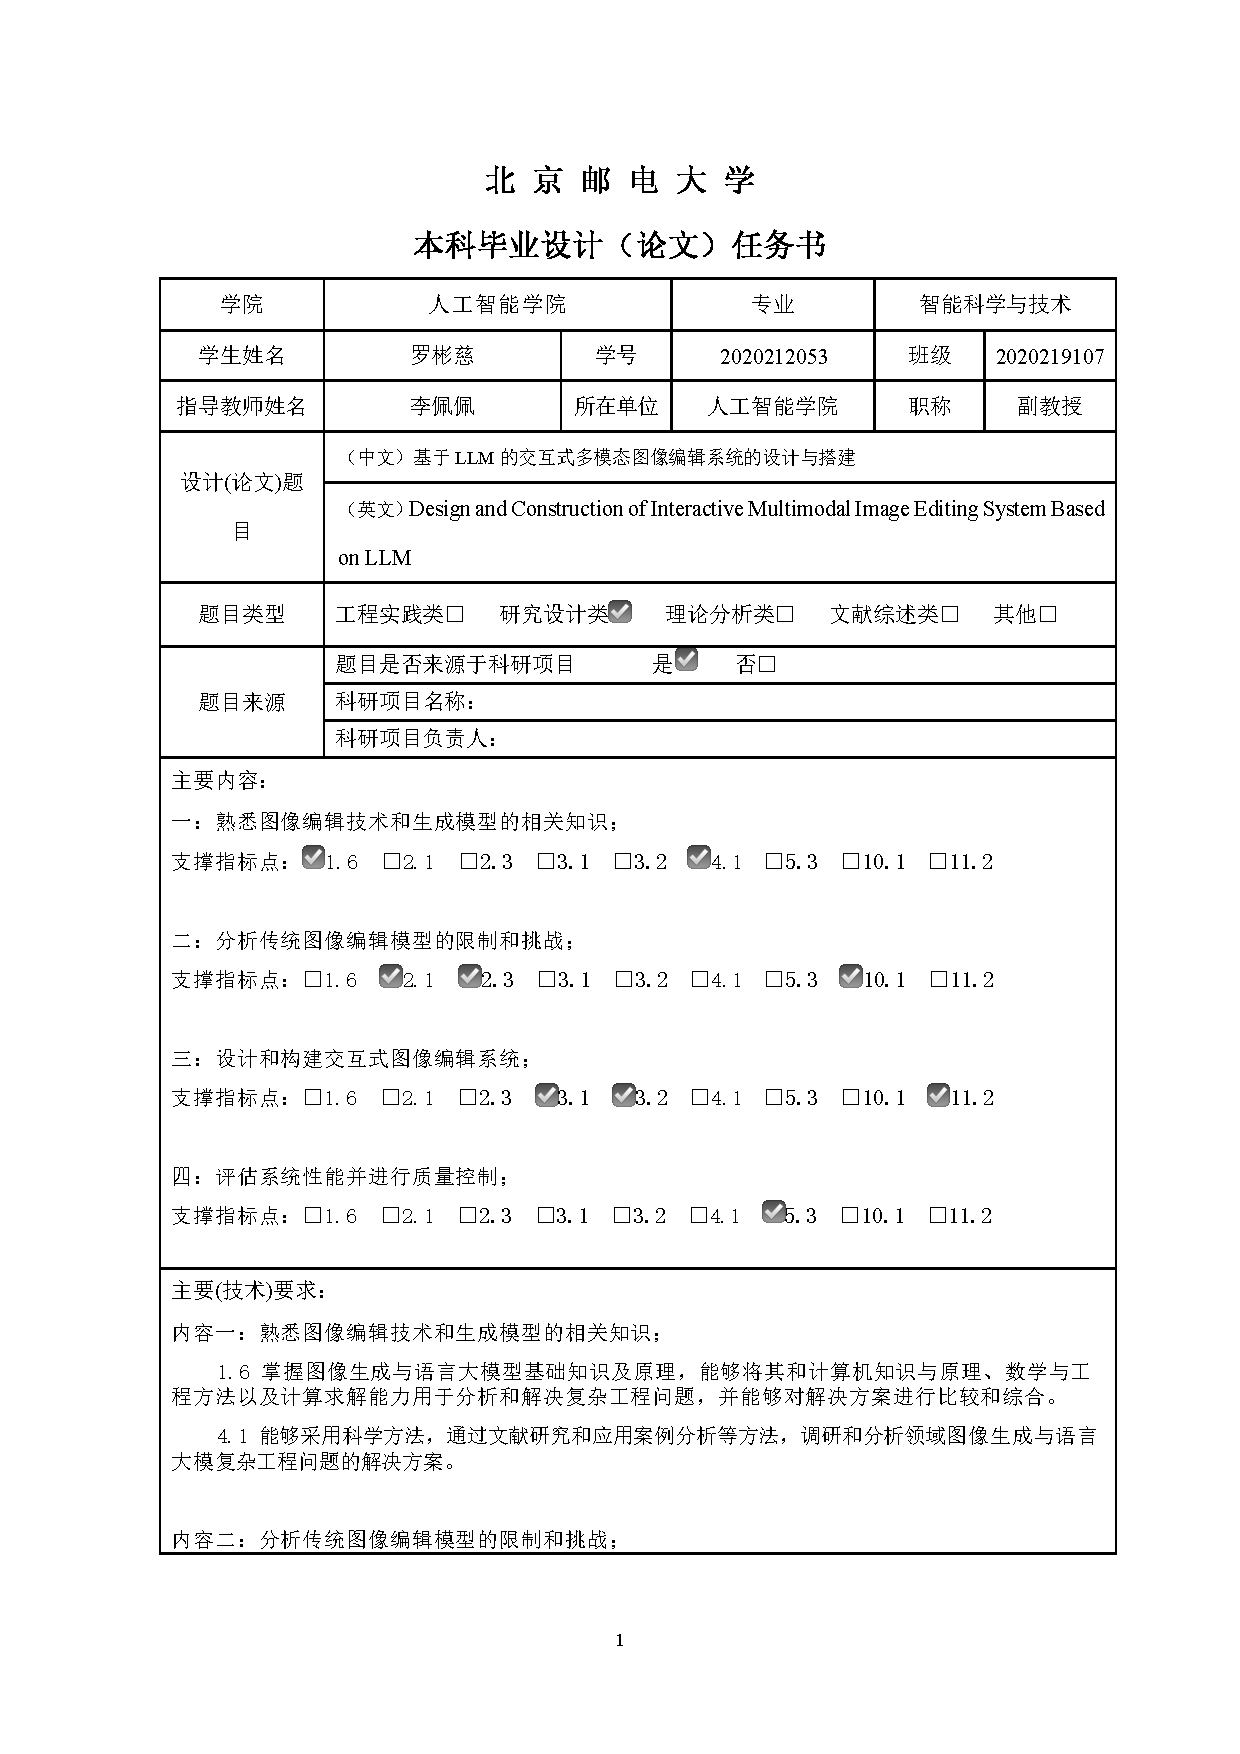
\includepdf[pages=-]{docs/task.pdf}  

% 成绩评定表
\blankmatter
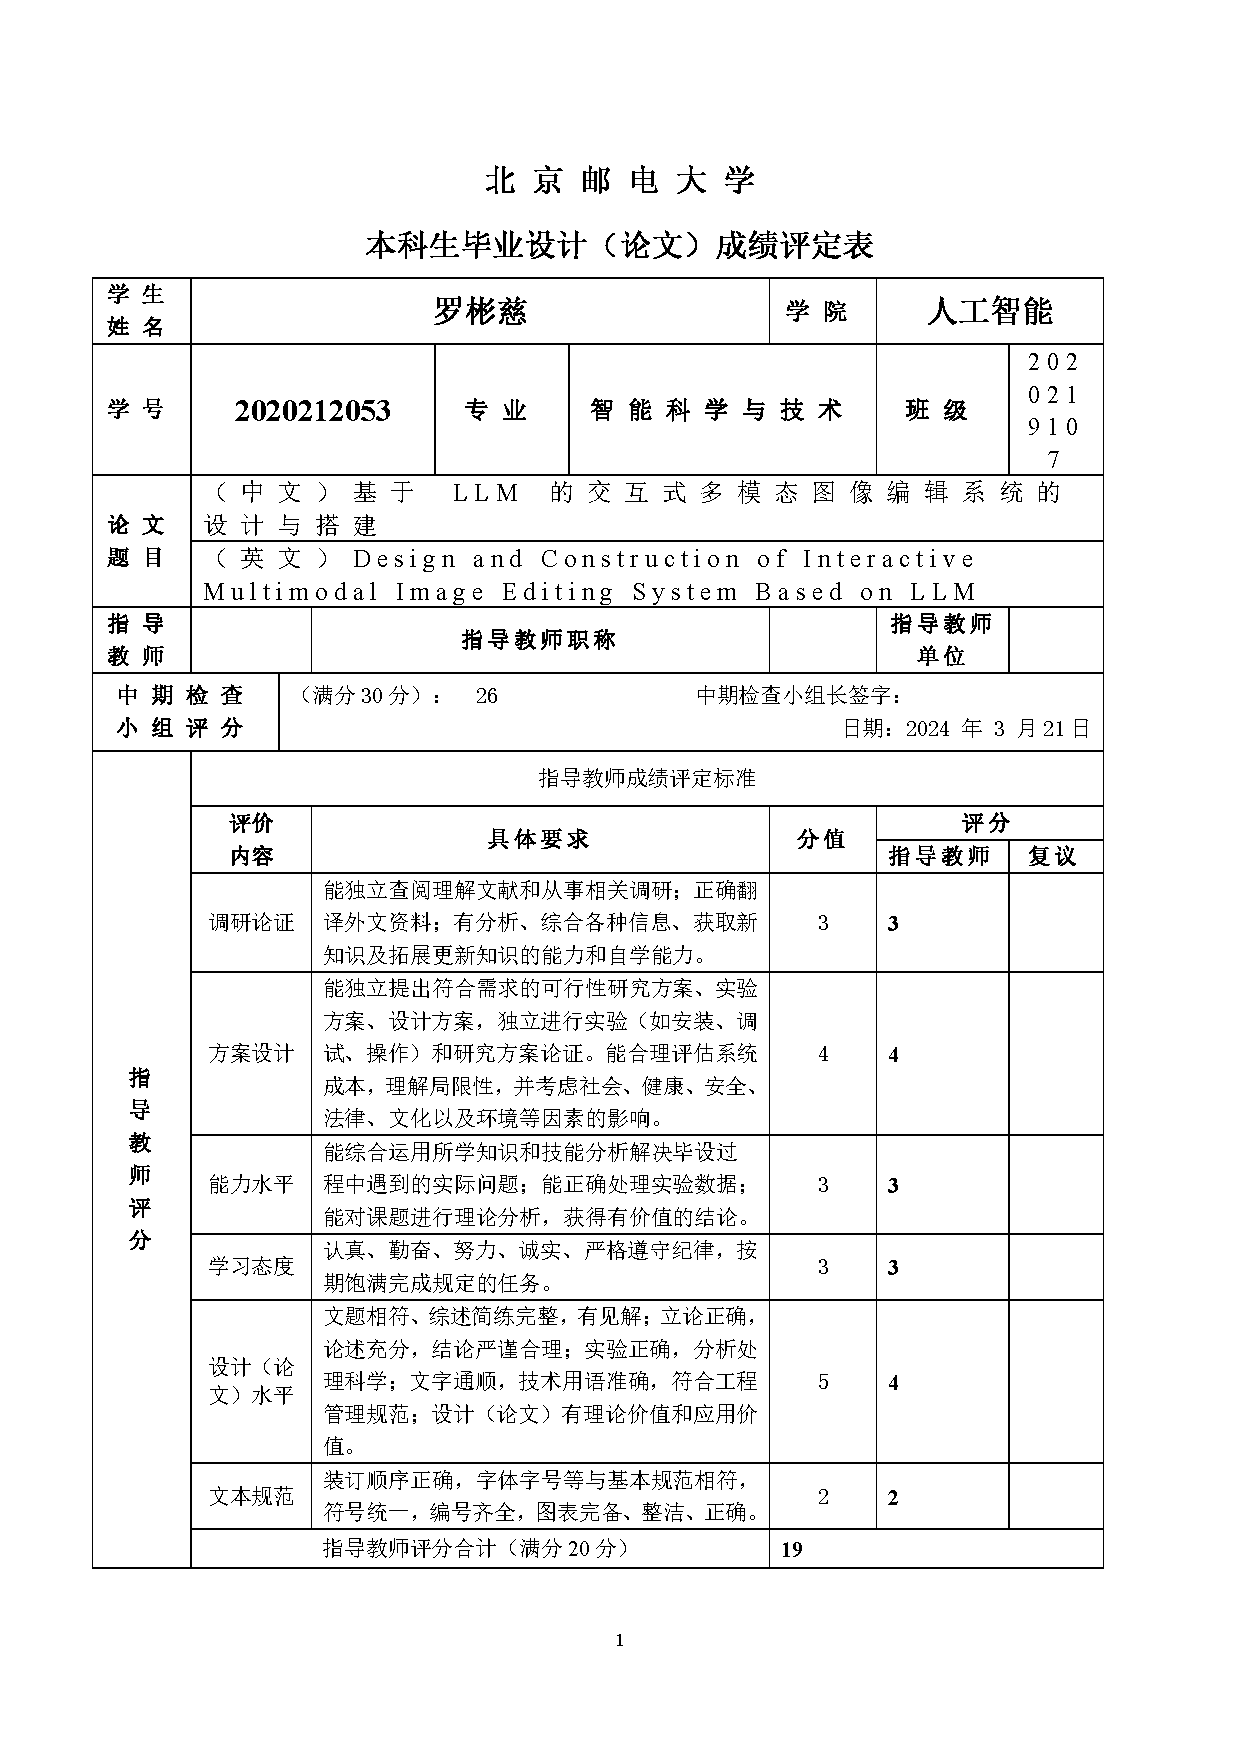
\includepdf[pages=-]{docs/scoreTable.pdf}  

% 诚信声明
\blankmatter

\includepdf[pages=-]{docs/statement.pdf} 

%%%%%%%%%%%%%%%%%%%%%%%%%%%%%%%%%%%%%%%%%%%%%%%%%%%%%%%%%%%%%%%%%%%%
%                                                                  %
%   Copyright (c) 2010 - 2011 Caspar Zhang <casparant@gmail.com>   %
%                                                                  %
%   This copyrighted material is made available to anyone wishing  %
%   to use, modify, copy, or redistribute it subject to the terms  %
%   and conditions of the GNU General Public License version 2.    %
%                                                                  %
%   This program is distributed in the hope that it will be        %
%   useful, but WITHOUT ANY WARRANTY; without even the implied     %
%   warranty of MERCHANTABILITY or FITNESS FOR A PARTICULAR        %
%   PURPOSE. See the GNU General Public License for more details.  %
%                                                                  %
%   You should have received a copy of the GNU General Public      %
%   License along with this program; if not, write to the Free     %
%   Software Foundation, Inc., 51 Franklin Street, Fifth Floor,    %
%   Boston, MA 02110-1301, USA.                                    %
%                                                                  %
%%%%%%%%%%%%%%%%%%%%%%%%%%%%%%%%%%%%%%%%%%%%%%%%%%%%%%%%%%%%%%%%%%%%

% 你只需要修改下面几行就可以完成大部分内容的填写,
% 这要求你具有一定的LaTeX基础,但是如果你足够聪明,
% 不具有LaTeX基础也可以完成。

% 论文中文题目
\def\thesistitle{基于LLM的交互式多模态图像编辑系统的设计与搭建}

% 论文英文题目
%提示:英文摘要页的标题注意格式要求。
\def\thesistitleen{Design and Construction of Interactive Multimodal Image Editing System Based on LLM}

% Thank Words
\def\thankwords{

致谢的内容。
}
    % Main items 
%%%%%%%%%%%%%%%%%%%%%%%%%%%%%%%%%%%%%%%%%%%%%%%%%%%%%%%%%%%%%%%%%%%%
%                                                                  %
%   Copyright (c) 2010 - 2011 Caspar Zhang <casparant@gmail.com>   %
%                                                                  %
%   This copyrighted material is made available to anyone wishing  %
%   to use, modify, copy, or redistribute it subject to the terms  %
%   and conditions of the GNU General Public License version 2.    %
%                                                                  %
%   This program is distributed in the hope that it will be        %
%   useful, but WITHOUT ANY WARRANTY; without even the implied     %
%   warranty of MERCHANTABILITY or FITNESS FOR A PARTICULAR        %
%   PURPOSE. See the GNU General Public License for more details.  %
%                                                                  %
%   You should have received a copy of the GNU General Public      %
%   License along with this program; if not, write to the Free     %
%   Software Foundation, Inc., 51 Franklin Street, Fifth Floor,    %
%   Boston, MA 02110-1301, USA.                                    %
%                                                                  %
%%%%%%%%%%%%%%%%%%%%%%%%%%%%%%%%%%%%%%%%%%%%%%%%%%%%%%%%%%%%%%%%%%%%

% 你只需要修改下面内容就可以完成中英文摘要,
% 这要求你具有一定的LaTeX基础,但是还是那句话,
% 如果你足够聪明,不具有LaTeX基础也可以完成。

% 中文摘要
\def\abstractzh{
%从这里开始写你的摘要,分段需要空一行。
随着深度学习技术在图像处理领域和文本生成领域的迅速发展,多模态交互系统的构建已成为研究的热点。本文介绍了一个基于最新图像生成模型和大语言模型的交互式多模态图像编辑系统的设计与搭建。系统利用了Stable Diffusion、DALL-E等图像生成模型和ChatGPT系列、ChatGLM2-6B等大语言模型,通过图形用户界面(GUI)、中间件(middleware)进行图像生成模型和大语言模型的整合,实现了一个既直观又高效的基于文本交互的多模态图像编辑系统。用户可以通过简单的文本指令控制图像编辑过程,系统能够自动解析这些指令并修改图像。本项目评估了系统在实际应用中的表现,结果显示该系统能够有效地提高图像编辑效率和用户交互体验。
%摘要结束
}

% 中文关键字 
% TODO: 改成可变长度的
\def\abszhkeyone{图像编辑}
\def\abszhkeytwo{大语言模型}
\def\abszhkeythree{多模态}
% \def\abszhkeyfour{模板}
% \def\abszhkeyfive{示例}

% ABSTRACT
\def\abstracten{
%Your abstract here, to make a new paragraph, give an extra blank line please.
With the rapid development of deep learning technology in the fields of image processing and text generation, the construction of multimodal interaction systems has become a hot topic of research. This paper introduces the design and construction of an interactive multimodal image editing system based on the latest image generation models and large language models. Utilizing image generation models such as Stable Diffusion and DALL-E, and large language models such as the ChatGPT series and ChatGLM2-6B, the system integrates these models through a graphical user interface (GUI) and middleware. This setup achieves an intuitive and efficient text-based multimodal image editing system. Users can control the image editing process through simple text commands, and the system can automatically parse these instructions and modify images. The project evaluated the system's performance in practical applications, and the results show that the system effectively improves image editing efficiency and user interaction experience.
%Abstract done
}

% Key Words 
% TODO: 改成可变长度的
\def\absenkeyone{Image Editing}
\def\absenkeytwo{Large Language Models}
\def\absenkeythree{Multimodal}
% \def\absenkeyfour{template}
% \def\absenkeyfive{example}


  % Abstract

\fancypagestyle{plain}{\pagestyle{frontmatter}}
\frontmatter
\tableofcontents % Content

% 正文
\newpage\mainmatter
\fancypagestyle{plain}{\pagestyle{mainmatter}}

%\let\cleardoublepagebak=\cleardoublepage
%\let\cleardoublepage\relax % Make new chapter stay on old page

%%%%%%%%%%%%%%%%%%%%%%%%%%%%% Main Area %%%%%%%%%%%%%%%%%%%%%%%%%%%%

\chapter{绪论} % 2085 + 66 + 25 = 2176
\section{项目背景}
随着技术的迅速发展,图像生成技术在多个行业中发挥着越来越重要的作用,尤其是在媒体娱乐、数字营销和智能医疗等领域。
然而,尽管其应用广泛,传统的图像编辑技术仍面临许多挑战,尤其是在交互性和生成图像质量上的限制。

传统图像编辑工具往往依赖于专业的技术知识和复杂的操作界面,这对于普通用户来说是一个较大的门槛。
用户需要花费大量时间学习如何使用这些工具,这限制了工具的普及性和易用性。这些工具的交互性通常较差,不能很好地根据用户的具体需求进行灵活调整和响应。

为了克服这些挑战,人们正在探索利用深度学习技术来改善图像编辑系统。
深度学习,特别是扩散模型,已经在图像生成领域显示出了巨大的潜力。
这些技术能够学习大量图像数据,自动提取复杂的特征,并生成高质量的图像。
此外,结合最新的GPT4Turbo等性能优异的大语言模型,可以进一步提升系统的交互性,实现更加自然和直观的用户界面。

图像生成模型是深度学习领域中一个活跃的研究方向,主要致力于通过机器学习技术生成高质量的图像。这些模型在多种应用场景中均有广泛应用,包括艺术创作、游戏开发、电影制作等。目前,图像生成模型主要包括生成对抗网络(GANs)、变分自编码器(VAEs)和扩散模型等。

扩散模型是近年来发展起来的一种新型生成模型,与传统的生成对抗网络(GANs)和变分自编码器(VAEs)相比,扩散模型在生成图像的质量和多样性方面展现出了卓越的性能。其基本原理是模拟从高质量数据分布到高熵噪声分布的逐步转变过程,然后再逆向这一过程以生成新的数据。
扩散模型的工作流程可以分为两个阶段:前向扩散过程和反向生成过程。在前向扩散过程中,模型逐渐将数据中的信息转化为噪声,这一过程通常通过向数据中逐步加入高斯噪声来实现。在反向生成过程中,模型则需要学习如何从噪声状态恢复出原始数据的分布,这一过程通常通过训练一个参数化的神经网络来完成,网络的目标是最小化原始数据与生成数据之间的差异。
扩散模型的关键优势在于其生成的图像具有较高的质量和自然性,这是因为模型在生成过程中能够更好地控制噪声的去除过程,并逐步精细化图像的细节。此外,扩散模型在训练过程中相对稳定,不易出现生成对抗网络中常见的模式崩溃问题。

大语言模型是人工智能领域中的一项核心技术,主要用于处理和理解自然语言。这些模型通过学习大量文本数据,能够生成文本、回答问题、翻译语言等。随着算力的提升和语料的增加,大语言模型已经取得了显著的进步,并在多个应用场景中展现出了巨大的潜力。
近几年,随着深度学习技术的发展,尤其是Transformers架构的提出,大语言模型的性能得到了质的飞跃。Transformers架构能够有效处理长距离依赖问题,并在许多自然语言处理任务中设定了新的性能标准,GPT(Generative Pre-trained Transformer)、BERT(Bidirectional Encoder Representations from Transformers)等主流模型,通过大规模的语料进行预训练,对语言的深层次结构和语义的理解能力有了显著的提升,在应用方面展现出广泛的适用性,包括但不限于文本生成、对话系统、语言翻译、内容摘要和情感分析等。

通过图像生成模型与大语言模型的结合,可以创建一个更加灵活且易用性强的图像编辑系统。
这样的系统不仅能够提供更加直观的编辑界面,降低用户的操作难度,还能够根据用户的描述自动生成或修改图像,
极大地提升生成图像的质量和编辑效率。例如,用户可以通过简单的语言指令,如“增加图片亮度”或“改变背景为海滩”,
直接与编辑系统交互,系统能够理解这些指令并即时作出响应。

通过整合深度学习和语言模型技术,我们有望构建出一个全新的交互式图像编辑系统。
这种系统不仅能够提供更高质量的图像编辑结果,更能够提供给用户更加自然的交互方式,为该领域的专业人士和普通用户都带来更多的可能性。
\section{项目意义}
通过融合先进的图像生成技术与大语言模型,本项目希望能搭建一个基于LLM的交互式图像编辑系统,提供更为易用、精准且高效的图像编辑工具,提升媒体娱乐、数字营销以及智能医疗等多个行业的图像处理能力。
通过实现更加智能化和用户友好型的编辑系统,为广大用户带来前所未有的图像编辑体验,并为促进技术创新做出贡献。这样的研究与开发,为图像编辑技术的未来提供了一种可能性和一条新的探索和实践路径。

\section{项目内容}
\buptfigure[width=0.7\textwidth]{pictures/arch.png}{}{arch_TMP}

% 该项目主要实现了GUI、middleware,并对Stable Diffusion和ChatGLM2-6B进行修改与适配。
% 各个模块之间的关系如 图1-1 所示。

% 通过在基于Stable Diffusion的开源项目stable-diffusion-webui上进行扩展,
% 本项目实现了通过API调用多种Stable Diffusion模型对图像进行修改的功能。

% 通过对ChatGLM2-6B进行微调,本项目实现了通过API调用针对本任务微调过的ChatGLM2-6B模型。

% 通过调用OpenAI的API,本项目实现了多个功能:通过GPT4V生成图像修改的建议、
% 通过GPT3.5Turbo辅助生成微调大语言模型的数据集和图像修改的指令、
% 通过DALL-E2实现在Stable Diffusion不可用时作为替代模型对图像进行修改。

% GUI主要通过python语言实现,其构建了一个直观、易于使用的用户交互界面。
% 在消耗大量计算资源的任务上,GUI会通过API对middleware发出请求,
% 减少了用户侧对计算资源的依赖,降低了用户的使用门槛。

% middleware使用golang语言搭建了一个后端服务,其接入了Stable Diffusion、ChatGLM2-6B、OpenAI的API,并将这些API进行整合后向GUI提供API。middleware的建立实现了一对多服务的能力,提高了GUI调用多方API的便利性,同时通过统一配置提高了系统的可维护性。

该项目是一个多模态交互式图像编辑系统,它主要实现了GUI、middleware、以及对Stable Diffusion和ChatGLM2-6B模型的修改与适配。在整体结构上,GUI、middleware、以及模型修改之间的相互关系和数据流向见 图1-1。

项目基于Stable Diffusion的开源项目stable-diffusion-webui进行了扩展,增强了其功能。系统可以调用不同的Stable Diffusion模型并结合多个扩展后的功能来对图像进行精细的修改和调整。这一功能的实现大大增强了系统对图像处理的灵活性和多样性。

项目还包括了对ChatGLM2-6B模型的微调。通过利用专门为本项目的需求生成的微调数据集进行微调,进一步提升了语言模型处理特定任务的能力和准确性,且能够利用API调用这些经过微调的ChatGLM2-6B模型。

通过调用OpenAI的API,本项目实现了多项功能:利用GPT4V生成关于图像修改的建议,使用GPT3.5Turbo来辅助生成用于微调大语言模型的数据集以及图像修改指令,以及在Stable Diffusion模型不可用时,使用DALL-E2作为替代模型来进行图像修改。这些功能为基于LLM的交互式图像编辑系统提供了强大的工具。

在GUI方面,本系统主要通过Python语言实现,构建了一个直观且用户友好的交互界面。该界面简洁易用,通过API调用向middleware发出请求,有效减轻了用户在执行计算密集型任务时对硬件资源的需求,从而降低了用户侧的使用门槛。

middleware部分使用Golang语言构建了一个后端服务。这个服务不仅接入了Stable Diffusion、ChatGLM2-6B、OpenAI的API,还将这些API进行了有效的整合,向GUI提供了一致风格的API接口。这种设计不仅提升了GUI调用多方API的便利性,也通过统一的配置和管理,极大地增强了系统的可维护性和稳定性。

\chapter{总体方案设计} % 1575+250 + 207 + 108 = 2140
\section{GUI}
GUI虽然承担计算任务较少,但却是承载本项目结构与逻辑的关键部分。通过使用符合规则的指令作为中枢,
GUI打通了大语言模型和图像生成模型之间的壁垒,使基于LLM的创新交互式图像编辑系统成为可能。GUI的模块构成如 表2-1 :
\begin{bupttable}{GUI模块}{table_gui_modules}
    \begin{tabular}{|l|l|}
        \hline \textbf{模块} & \textbf{描述} \\
        \hline BaseImage & 接受上传的原始图片并预览  \\
        \hline EditedImage & 预览修改后的图片 \\
        \hline Operation Board & 执行指令  \\
		\hline Settings & 对系统进行设置  \\
		\hline Chat & 与大语言模型交互的聊天界面  \\
		\hline Edit Image & 对图像进行自定义遮罩和换脸等操作  \\
		\hline Auto & 执行自动化操作  \\
		\hline Manual & 系统使用说明  \\
        \hline
    \end{tabular}
\end{bupttable}

用户首先上传需要修改的图片,然后可在Chat模块中选择不同的大语言模型进行交互并得到相应的指令,
最后在Operation Board模块中选择指令执行或一键全部执行。如果对自动生成的遮罩不满意,
可在Edit Image中对遮罩进行修改。

在Auto模块中,用户可通过选择多张图片批量生成满足微调大语言模型微调所需的数据。
其会循环地从给定的图片集中随机选择图片继续分割,将分割后的结果和特定的prompt通过GPT3.5Turbo生成对应的修改建议,
再将分割的结果、生成的建议通过GPT3.5Turbo生成指令。

\section{middleware}
middleware是项目的核心组件,通过整合多个平台的API,为GUI提供统一的、简单易接入的API服务。其主要特点包括但不限于:
1. API整合:middleware整合了多个平台的API,包括图像生成模型、语言模型等,使得GUI可以通过统一的接口调用不同功能模块;
2. 统一风格:middleware设计了统一的API风格和路由规范,使得GUI可以轻松使用API服务,提高开发效率;
3. 简单易接入:middleware提供了简单易用的API服务,GUI无需关注具体实现细节,只需按照简单的请求规范调用API即可;
4. 稳定性和可靠性:middleware基于Golang语言实现,具有高效的并发处理能力和稳定的运行性能,保证了API服务的稳定性和可靠性;
5. 易于维护:middleware采用了Beego框架,具有清晰的代码结构和模块化设计,易于维护和扩展,保证了项目的长期可持续发展。
其向GUI提供的主要API如 表2-2 所示:
\begin{bupttable}{middleware 主要API}{table_gui_modules}
    \begin{tabular}{|l|l|l|}
        \hline \textbf{API} & \textbf{路由} & \textbf{描述} \\
        \hline PostSDTxt2Img & /v1/pics/txt2img & 通过Stable Diffusion模型生成图片  \\
        \hline PostSDImg2Img & /v1/pics/img2img & 通过Stable Diffusion模型修改图片 \\
        \hline PostDALLE2Edit & /v1/pics/openai/img2img & 通过DALL-E2模型修改图片  \\
		\hline GetLoras & /v1/pics/loras & 获取可用的LoRa模型列表  \\
		\hline PostHuggingFaceImgSegment & /v1/pics/huggingface/segment & 获取图像分割结果  \\
		\hline PostGPT3Dot5Turbo & /v1/chat/gpt3dot5turbo & 调用GPT3.5Turbo  \\
		\hline PostGPT4Turbo & /v1/chat/gpt4 & 调用GPT4Turbo  \\
		\hline PostChatGLM2\_6B & /v1/chat/glm2\_6b & 调用ChatGLM2-6B  \\
		\hline PostGPT4V & /v1/chat/gpt4v & 调用GPT4V  \\
        \hline
    \end{tabular}
\end{bupttable}

\section{Stable Diffusion}
Stable Diffusion 是一种基于扩散模型的深度学习图像生成模型,它能够根据文本描述生成高质量的图像。
这个模型采用了条件生成技术,允许用户通过文本指令来引导图像的生成,使其在艺术创作、媒体娱乐、广告和数字营销等多个领域具有广泛的应用。
其核心在于从噪声逆向还原生成高质量的图片。

sd-webui-controlnet\footnote{https://github.com/Mikubill/sd-webui-controlnet}使用了ControlNet\cite{zhang2023adding}的原理,
旨在增强原有 Stable Diffusion 模型的图像生成控制能力。通过集成一个额外的控制网络(ControlNet),
允许用户精确指导图像的具体内容,显著提升了生成图像的细节质量和一致性。

sd-webui-roop\footnote{https://github.com/s0md3v/sd-webui-roop}基于DeepFake\cite{van2021deepfake},
允许用户在图片中进行面部替换,简化了面部交换的过程,无需训练特定的模型,大大降低了使用复杂度。

由于本项目对于图像生成模型的要求较高且需求复杂,为了便于结合Stable Diffusion模型和其他前沿研究成果及开源社区项目,本项目在构建Stable Diffusion模块时
以开源项目stable-diffusion-webui\footnote{https://github.com/AUTOMATIC1111/stable-diffusion-webui}为基础,
结合sd-webui-controlnet和sd-webui-roop等扩展,通过 API 为middleware提供服务。

\section{OpenAI}
本项目使用了OpenAI\footnote{https://openai.com}的GPT3.5Turo、GPT4Turbo、GPT4V、DALL-E2等模型,通过 API 调用OpenAI的模型。

GPT-3.5 Turbo 是 OpenAI 开发的一款先进的自然语言处理模型,属于 GPT-3 系列的增强版本。这个模型在处理大量文本和生成文本方面表现出色,适用于聊天机器人、内容创作、文本摘要等应用。GPT-3.5 Turbo 优化了处理速度和响应时间,提高了交互效率。

GPT-4 是 GPT-3 的后续版本,代表了最新一代的语言预测和生成技术。它在模型结构和训练数据量上进行了大幅扩展,使其能够更准确地理解和生成复杂的文本。GPT-4 在理解上下文、维持一致性以及生成更自然的语言方面具有显著优势。

GPT-4V 是 GPT-4 的一个特殊版本,专门优化用于视觉任务,比如图像标注、视觉问答等。这个版本结合了文本和视觉处理能力,能够更好地理解和生成与图像相关的文本内容。

DALL-E 2 是一个先进的图像生成模型,专门设计用来创建新颖的图像和艺术作品。它可以根据用户提供的文本描述生成详细、高质量的图像。DALL-E 2 的核心优势在于其创造力和多样性,能够在遵循描述的同时,创造出独特和富有创意的视觉内容。

\section{ChatGLM2-6B}
ChatGLM2-6B是由清华大学开发的第二代开源双语(中英)对话模型,基于ChatGLM-6B的成功经验并引入了多项新特性和性能提升。
这款模型经过大规模预训练,实现了显著的性能提升,并在多个数据集上表现出色。
ChatGLM2-6B支持更长的对话上下文,并提高了推理速度和降低了显存占用,
使得即使在资源有限的环境下也能有效运行。

本项目使用ChatGLM2-6B模型,使用开源项目LLaMA-Factory\footnote{https://github.com/hiyouga/LLaMA-Factory},
利用本项目提供的数据自动生成功能所生成的数据集,使用LoRa\cite{hu2021lora}方法对模型进行微调以在本项目所需的任务中获得更佳的表现。微调后的模型通过fastapi提供 API 服务。


\chapter{GUI的构建} % 1674 + 257 + 139 = 2070
在本项目中,GUI作为关键组成部分,虽仅承担极少的计算任务,却在结构与逻辑上起着至关重要的作用。
它通过使用标准化的指令连接大语言模型和图像生成模型,实现了基于LLM的创新交互式图像编辑系统。
用户首先上传原始图片至BaseImage模块进行预览,之后可通过Chat模块与大语言模型进行交互,获取编辑指令。
用户可以在Operation Board模块中选择单独或批量执行这些指令。
若对自动生成的遮罩不满意,可在Edit Image模块中手动调整。
此外,Auto模块允许用户批量处理多张图片,自动生成数据以微调大语言模型。
该过程包括图片的自动分割、利用GPT3.5Turbo生成编辑建议及相应的执行指令。
这样的设计不仅提升了系统的效率,也优化了用户的交互体验。
\section{图像自动遮罩与优化}
由于本项目需要提供对图像进行部分修改的功能,所以需要在使用图像生成模型进行图像编辑时需要提供一个遮罩以明确需要修改的部分和不需要修改的部分。
为了自动生成符合要求的遮罩,本项目借助图像分割和大语言模型的辅助,可通过两种方式生成自动遮罩:基于关键词对自动生成遮罩和基于已给出的点自动填充生成遮罩。
两种方法都会首先使用图像分割模型对图像进行分割(如图3-1),然后根据给出的要求对相应的部分进行遮罩生成原始的遮罩。受制于图像分割模型在边缘上的表现并不理想,
需要对特定的分割部分进行处理以提高遮罩的质量,因此最后会通过本项目设计的优化算法生成最终的遮罩。
\begin{figure}[!htbp]
    \centering
    \subfloat[]{ %[]对齐方式,t为top,b为bottom,留空即可
	\label{Fig:SegmentOrigin1} % 子图1标签名
    	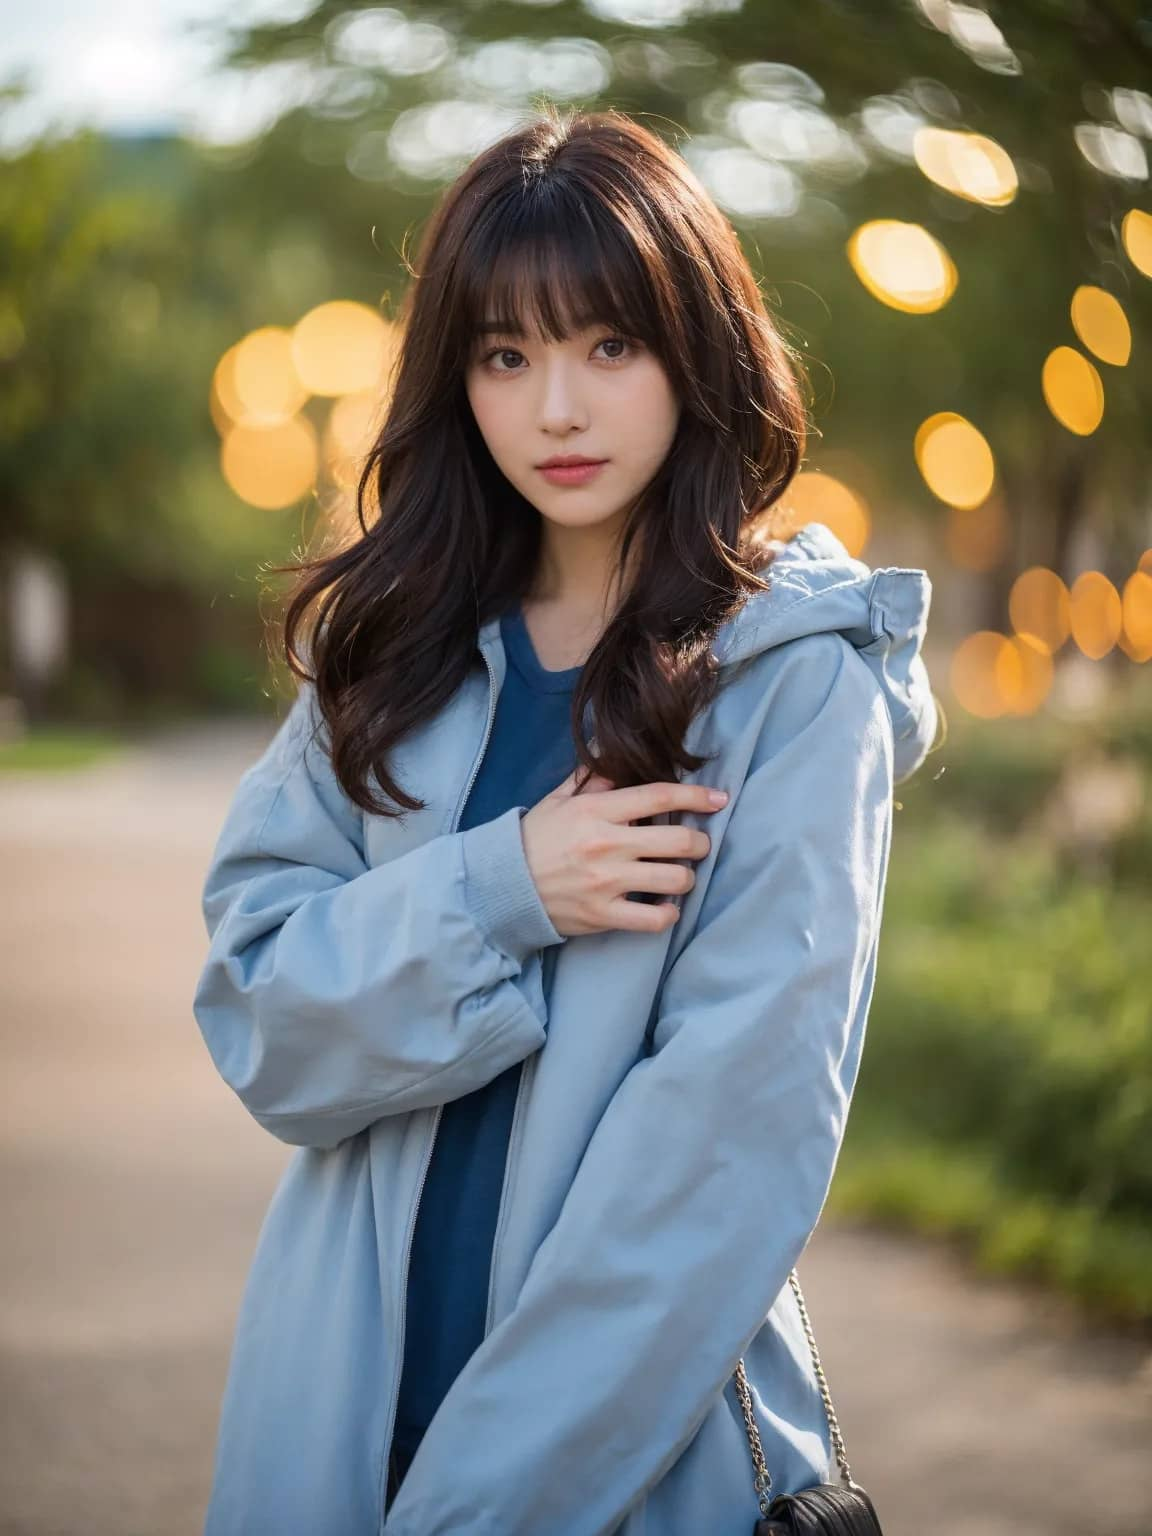
\includegraphics[width=0.24\textwidth]{pictures/example1_origin} %插入图片命令,格式为[配置]{图片路径}
    }
    \quad %空格
    \subfloat[]{
	\label{Fig:SegmentResult1} % 子图2标签名
    	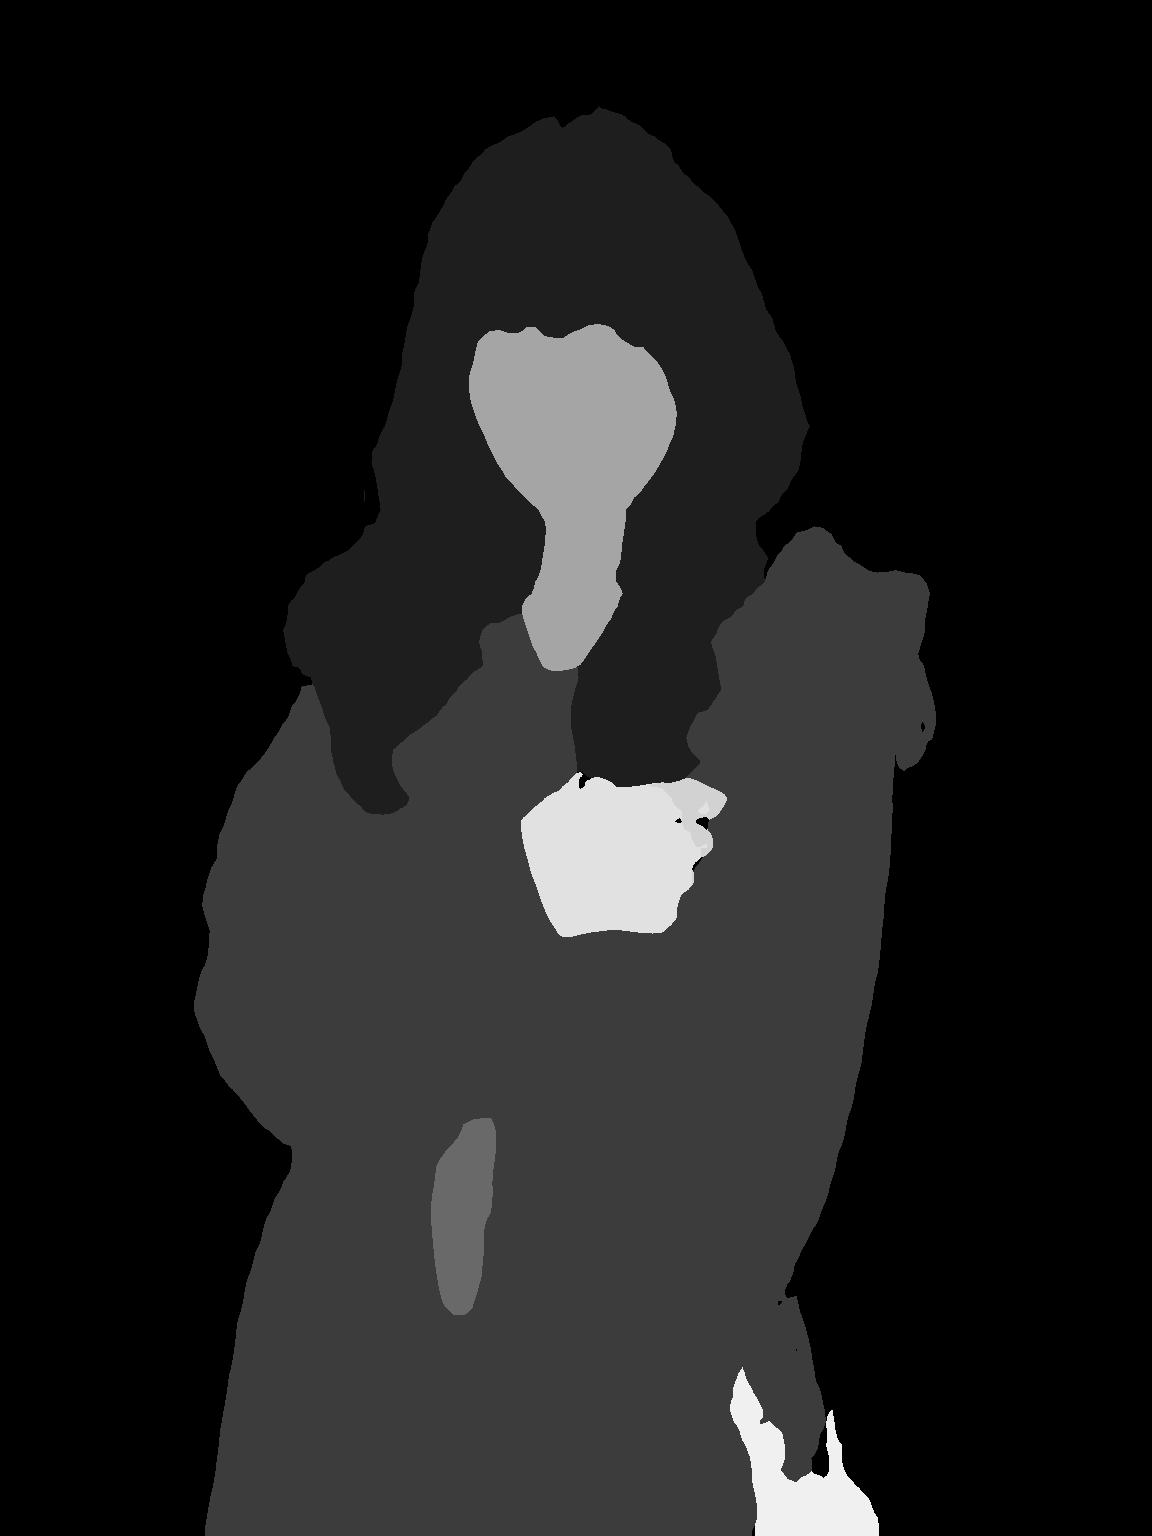
\includegraphics[width=0.24\textwidth]{pictures/example1_segment}
    }
    \caption{图像分割结果:\protect\subref{Fig:SegmentOrigin1}原始图像,\protect\subref{Fig:SegmentResult1}分割结果} %注意须使用\protect\subref{}进行标号引用
    \label{Fig:Segment} % 整个组图的标签名
\end{figure}

\subsection{图像自动遮罩}
基于关键词自动生成遮罩的方法会根据关键词和图像分割结果生成自动原始的遮罩,该功能会遍历每个给出的关键词,
若关键词与分割结果之一吻合,则会对相应的分割区域进行遮罩,生成原始的遮罩(如图3-2)。
\begin{figure}[!htbp]
    \centering
    \subfloat[]{ %[]对齐方式,t为top,b为bottom,留空即可
	\label{Fig:SegmentOrigin2} % 子图1标签名
    	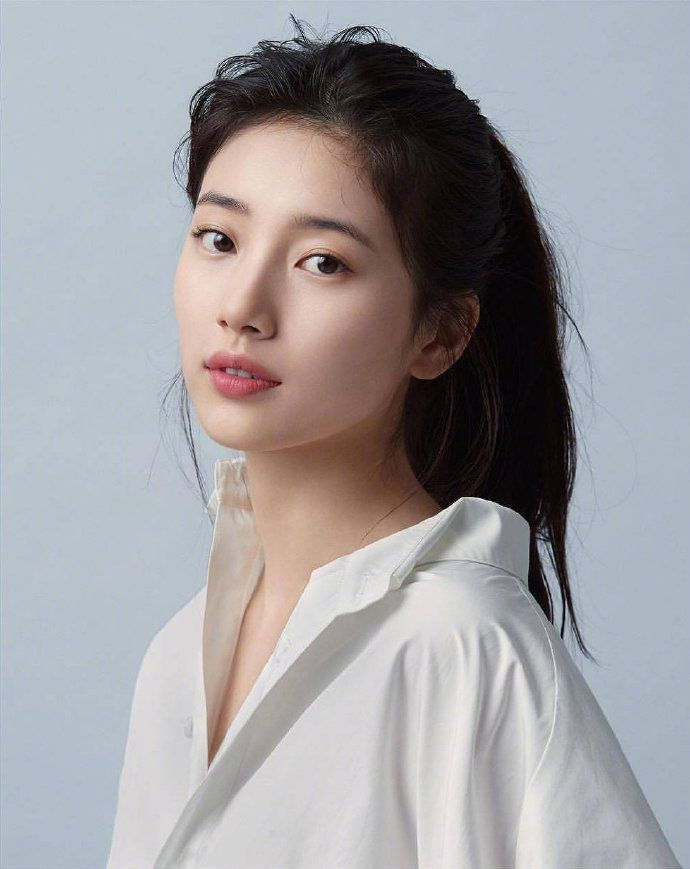
\includegraphics[width=0.24\textwidth]{pictures/example2_origin} %插入图片命令,格式为[配置]{图片路径}
    }
    \quad %空格
    \subfloat[]{
	\label{Fig:SegmentResult2} % 子图2标签名
    	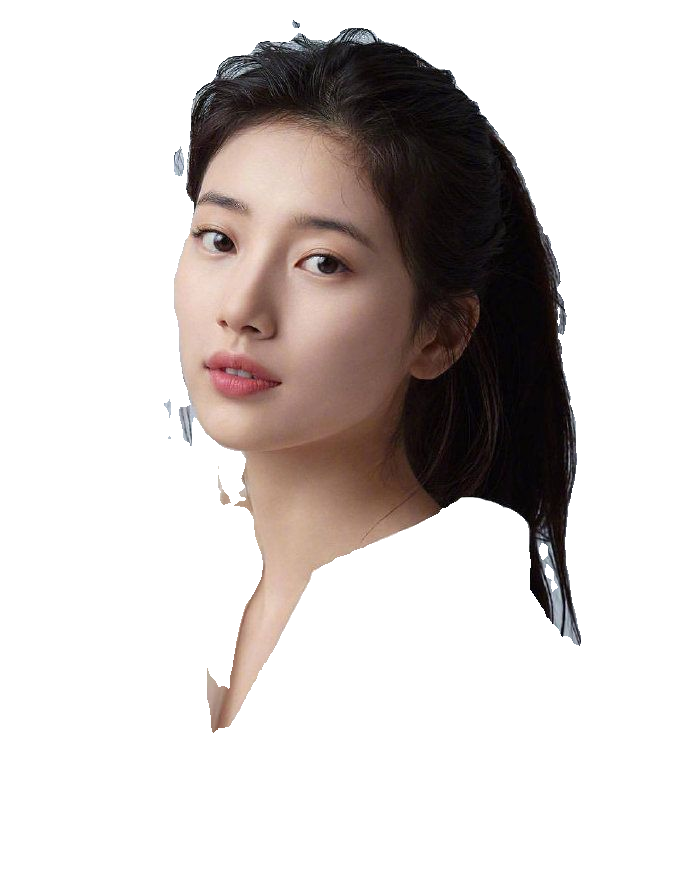
\includegraphics[width=0.24\textwidth]{pictures/example2_step1}
    }
    \caption{关键词自动生成遮罩结果:\protect\subref{Fig:SegmentOrigin2}原始图像,\protect\subref{Fig:SegmentResult2}kewords=['Background', 'Upper-clothes', 'Dress', 'Right-arm']得到的遮罩} %注意须使用\protect\subref{}进行标号引用
    \label{Fig:SegmentKeywords} % 整个组图的标签名
\end{figure}

基于已给出的点自动填充生成遮罩的方法会根据在图片中标记的点和图像分割结果生成自动原始的遮罩,该功能会遍历每个给出的点,
将该点所在的部分全部进行遮罩,最后生成原始的遮罩(如图3-3)。
\begin{figure}[!htbp]
    \centering
    \subfloat[]{
	\label{Fig:SegmentPoints} 
    	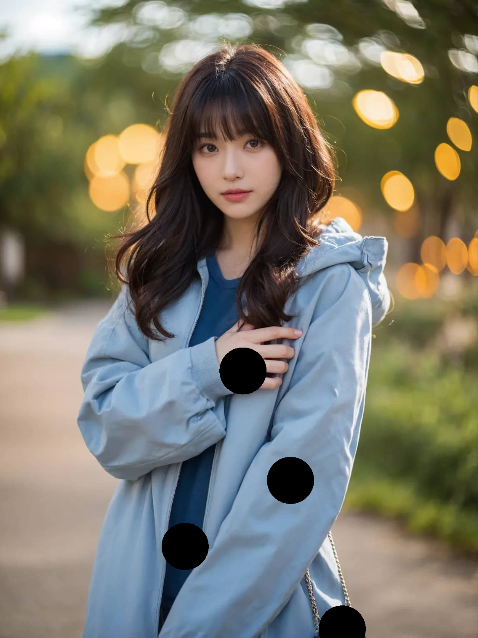
\includegraphics[width=0.24\textwidth]{pictures/example1_points}
    }
    \quad %空格
    \subfloat[]{
	\label{Fig:SegmentStep1} 
    	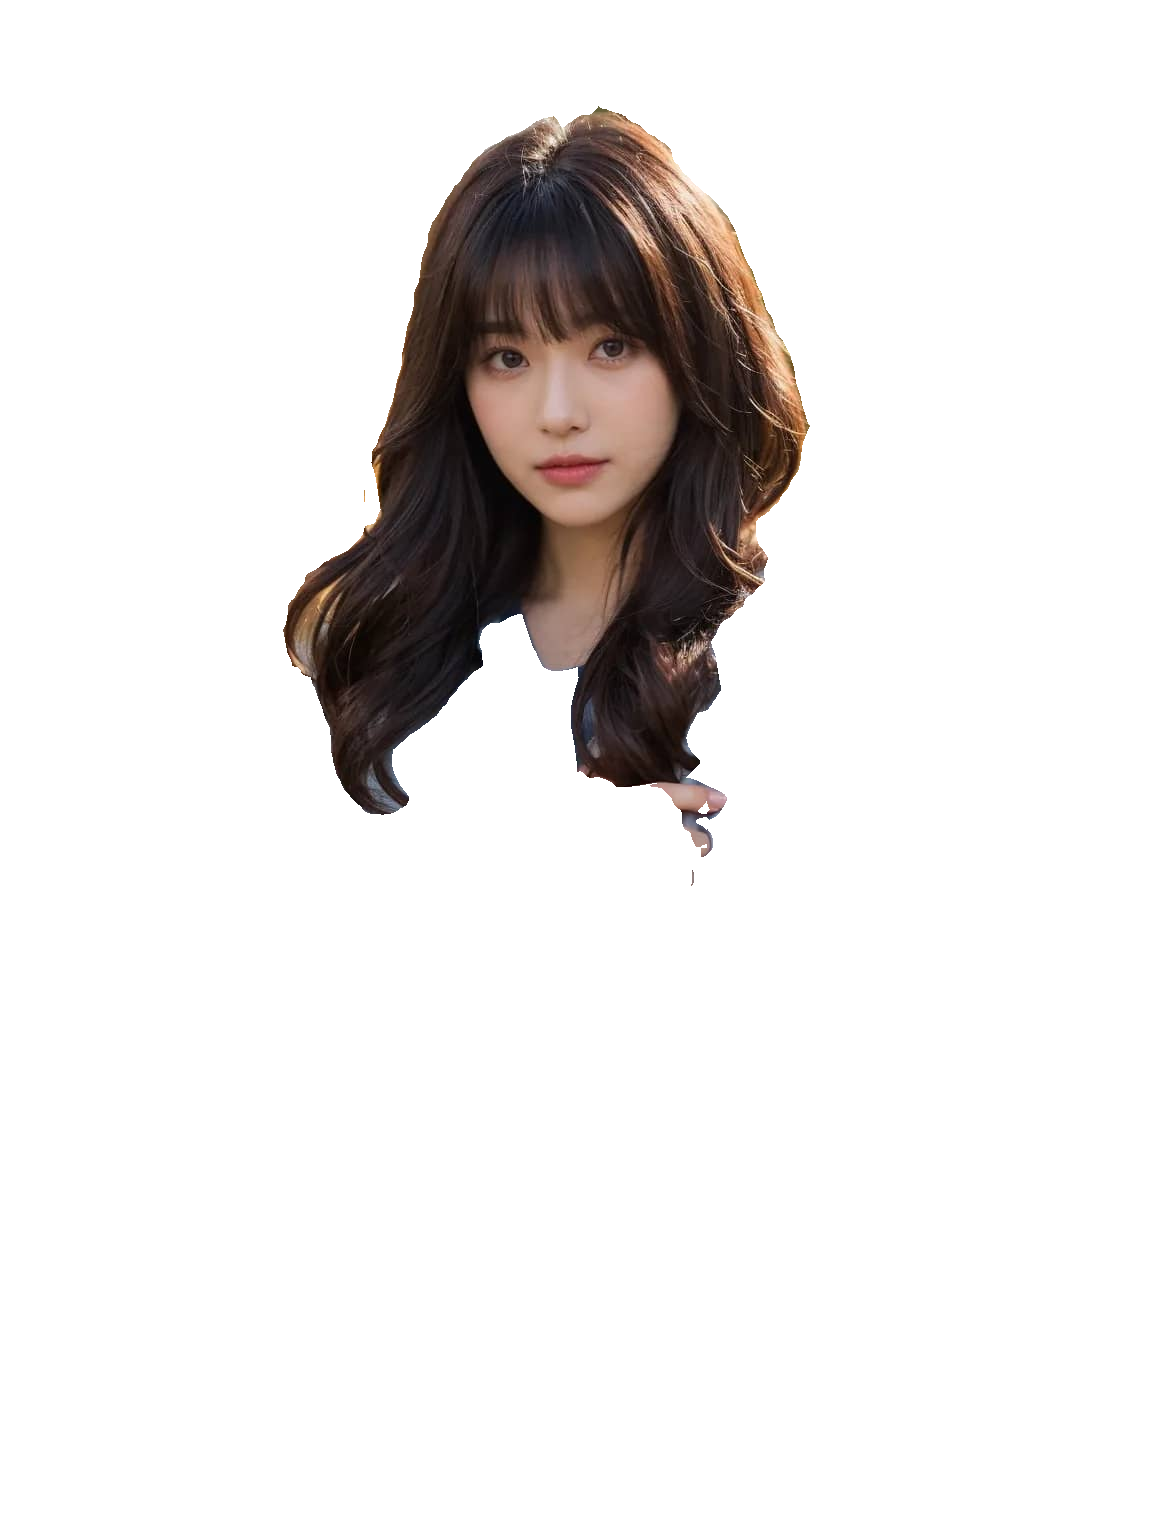
\includegraphics[width=0.24\textwidth]{pictures/example1_step1}
    }
    \caption{基于已给出的点自动填充生成遮罩:\protect\subref{Fig:SegmentPoints}标记后的图像,\protect\subref{Fig:SegmentStep1}生成的遮罩} %注意须使用\protect\subref{}进行标号引用
    \label{Fig:Point} 
\end{figure}

\newpage
\subsection{对自动生成的遮罩进行优化}
由于分割模型性能的限制,生成的原始遮罩可能在某些细节上表现不佳而影响图像编辑模型的结果,因此设计了一个算法对自动生成的遮罩
进行优化。该算法可以根据配置文件的设置,对特定的未被遮罩的部分在遮罩的边缘进行收缩。

\begin{algorithm} 
	\begin{spacing}{1.3}
		\floatname{algorithm}{算法}
		\caption{遮罩优化算法} 
		\label{MaskOptimizationAlgorithm}
		\renewcommand{\algorithmicrequire}{\textbf{输入:}}
		\renewcommand{\algorithmicensure}{\textbf{输出:}} 
			\begin{algorithmic}[1] 
				\Require 原始遮罩$OriginMask$,图像分割结果$SegmentResult$,配置文件$Config$
				\Ensure 优化后的遮罩$OptimizedMask$
				\State 获取遮罩与非遮罩的描边得到像素$EdgePixcels$
				\State 从配置文件和图像分割结果获取$ConfigPixcels$
                \State 仅保留出现在$EdgePixcels$中的$ConfigPixcels$
                \For{$pixcel$ in $ConfigPixcels$}
                    \State Apply MinFilter $Kernel$(in $Config$) in $OriginMask$[$pixcel$]
                \EndFor
                \State 得到优化后的遮罩$OptimizedMask$
			\end{algorithmic}
	\end{spacing}
\end{algorithm}

由于该算法仅会对遮罩边缘上的像素进行卷积且在设计时充分考虑到了内存中像素的存储顺序的原因,虽然需要复杂的处理过程,但经过多次的迭代后算法的时间复杂度降低至$O(mnr)$($m$,$n$表示图片的长宽,$r$表示设置的优化强度)。算法实现的效果如 图3-4 所示,可见在发丝附近遮罩的质量得到了明显的改善。
\begin{figure}[!htbp]
    \centering
    \subfloat[]{ %[]对齐方式,t为top,b为bottom,留空即可
	\label{Fig:MaskOrigin} % 子图1标签名
    	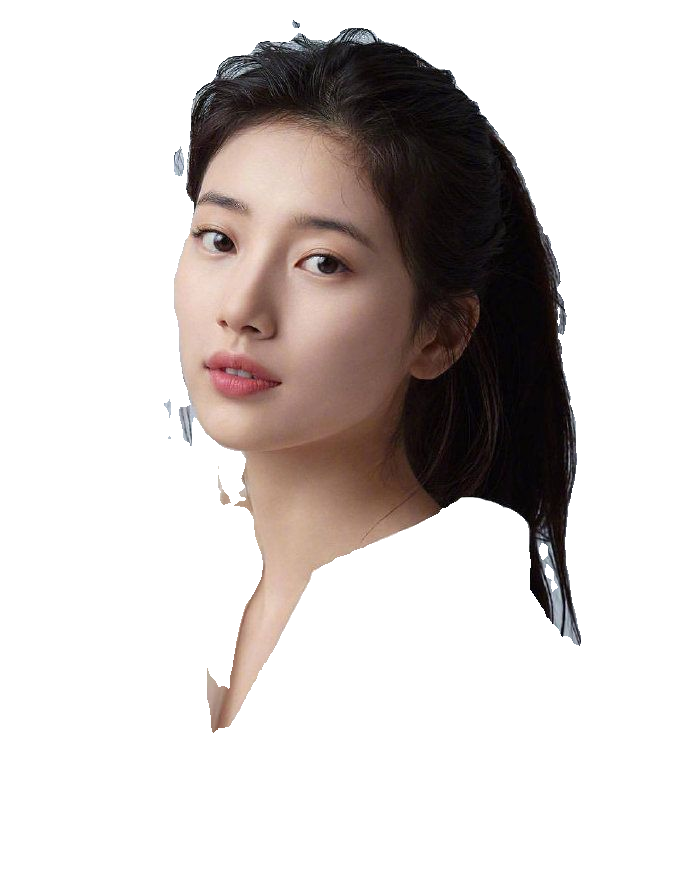
\includegraphics[width=0.24\textwidth]{pictures/example2_step1} %插入图片命令,格式为[配置]{图片路径}
    }
    \quad %空格
    \subfloat[]{
	\label{Fig:MaskOptimized} % 子图2标签名
    	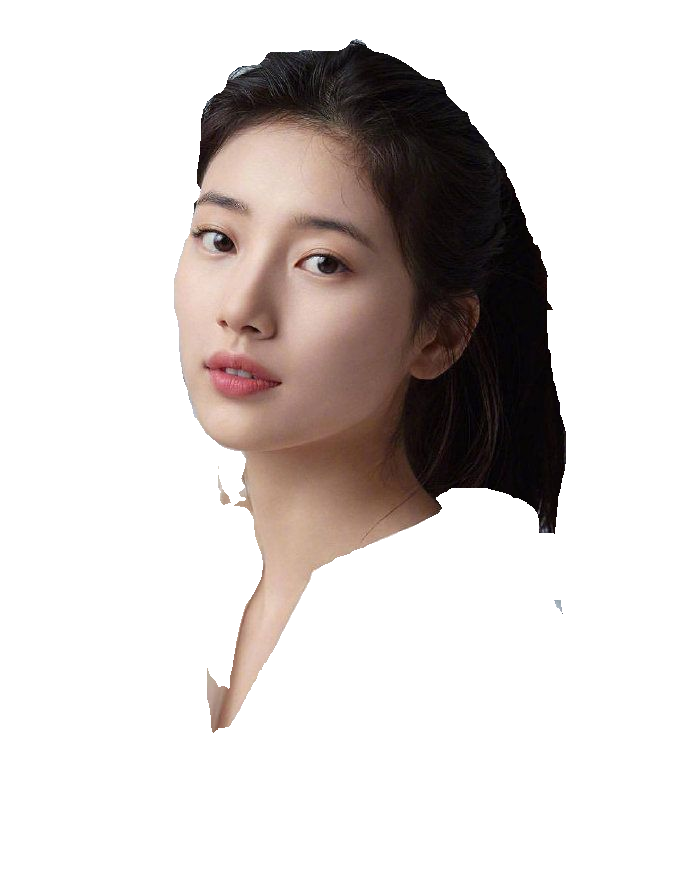
\includegraphics[width=0.24\textwidth]{pictures/example2_step2}
    }
    \caption{遮罩优化结果:\protect\subref{Fig:MaskOrigin}原始遮罩,\protect\subref{Fig:MaskOptimized}算法优化后的遮罩} %注意须使用\protect\subref{}进行标号引用
    \label{Fig:MaskOptimize} % 整个组图的标签名
\end{figure}
\newpage
\section{多模态}
如何打通大语言模型和图像生成模型是本项目的关键。本项目通过特定的prompt和图像分割结果,使用大语言模型生成JSON格式的指令并校验,并支持多轮对话。
用户可有选择性地执行生成的指令或执行全部指令。系统首先会按照给定的规则对指令进行预处理和排序,然后通过指令生成请求参数来调用图像生成模型。多模态任务的实现方式如图3-5。
\buptfigure[width=1\textwidth]{pictures/multimodal.png}{}{multimodal_TMP}

\subsection{JSON指令生成}
JSON(JavaScript Object Notation)是一种轻量级的数据交换格式,易于人阅读和编写,同时也易于机器解析和生成。
它基于JavaScript的一个子集,但独立于语言,被广泛应用于许多编程语言中。JSON主要用于网络应用间浏览器与服务器之间的数据传输。
在JSON中,数据以键值对的形式存在,可以表示数组、布尔值、数字、对象或字符串。由于其简洁性和易于交互的特性,JSON已成为Web应用中数据交换的主流技术。
由于JSON应用范围广且大语言模型JSON处理能力较强,本项目采用此格式来承载大语言模型和图像生成模型的联系。

通过特定的prompt和图像分割结果以及用户输入的修改意图,本项目可使用GPT3.5Turbo、GPT4Turbo、
微调后的ChatGLM2-6B生成JSON指令。例:当图像分割结果为$Background, Hair, Upper-clothes, Dress, Face, Right-arm$,用户输入为
“将背景更换为蓝天白云,将衣服更改为白色的T-shirt”时,生成的JSON指令如 代码3-1 所示。

\begin{lstlisting}[language=Python, caption=生成的指令, label=plus, tabsize=2]  
    [
        {
            "command" : "change",
            "paras" : [ ["Background","Upper-clothes"] , "blue sky, white T-shirt"]
        }
    ]
\end{lstlisting} 

\subsection{JSON指令校验}
由于大语言模型生成指令不稳定,需要对生成指令的合规性进行校验。校验规则存储为一个JSON文件,以修改非面部和面部的指令为例,校验规则如 代码3-2 所示:
\begin{lstlisting}[language=Python, caption=指令校验规则, label=plus, tabsize=2]  
    {
    "face": {
        "paras_type": [
            "<class 'str'>"
        ],
        "paras_enum": null,
        "paras_min": null,
        "paras_max": null,
        "combine": true,
        "priority": 1
    },
    "change": {
        "paras_type": [
            "<class 'list'>",
            "<class 'str'>"
        ],
        "paras_enum": null,
        "paras_min": null,
        "paras_max": null,
        "combine": true,
        "priority": 1
    }
}
\end{lstlisting} 
指令校验的算法如 算法-2 所示。
\begin{algorithm} 
	\begin{spacing}{1.3}
		\floatname{algorithm}{算法}
		\caption{JSON指令校验算法} 
		\label{JsonCommandCheckAlgorithm}
		\renewcommand{\algorithmicrequire}{\textbf{输入:}}
		\renewcommand{\algorithmicensure}{\textbf{输出:}} 
			\begin{algorithmic}[1] 
				\Require 待校验的指令$JsonCommands$、校验规则$Rules$
				\Ensure 校验后的指令$ValidJsonCommands$
                \For{$Command$ in $JsonCommands$}
                    \If {$Command$ satisfy $Rules$}
                        \State Add $Command$ to $ValidJsonCommands$
                    \EndIf
                \EndFor
			\end{algorithmic}
	\end{spacing}
\end{algorithm}

\subsection{多指令处理}
由于一次执行可能会涉及到多个指令,会遇到指令重复、指令优先性等问题,所以会对需要执行的指令进行合并与排序。
指令合并的算法如下:
\begin{algorithm} 
	\begin{spacing}{1.3}
		\floatname{algorithm}{算法}
		\caption{多指令处理算法} 
		\label{JsonCommandsProcessingAlgorithm}
		\renewcommand{\algorithmicrequire}{\textbf{输入:}}
		\renewcommand{\algorithmicensure}{\textbf{输出:}} 
			\begin{algorithmic}[1] 
				\Require 待处理的指令$OriginCommands$、指令合并规则$Rules$、指令优先性$Priority$
				\Ensure 处理后的指令$ProcessedCommands$
                \For{$Command$ in $OriginCommands$}
                    \If {Same $Command$ type already in $ProcessedCommands$}
                        \State Combine $Command$ to the same one in $ValidJsonCommands$ use $Rules$
                    \EndIf
                \EndFor
                \State 根据$Priority$对$ValidJsonCommands$进行排序
			\end{algorithmic}
	\end{spacing}
\end{algorithm}

\subsection{图像模型请求参数生成}
图像模型请求参数生成较为复杂,对于某个参数,其可能来源于GUI中可修改的设置,可能来源于指令,可能来源于模版,否则设置为默认参数。
由于每个参数来说,其来源的优先性可能不一致,因此设计了 算法-4 来生成图像模型请求参数。
\begin{algorithm} 
	\begin{spacing}{1.3}
		\floatname{algorithm}{算法}
		\caption{图像模型请求参数生成算法} 
		\label{ImageParasGenAlgorithm}
		\renewcommand{\algorithmicrequire}{\textbf{输入:}}
		\renewcommand{\algorithmicensure}{\textbf{输出:}} 
			\begin{algorithmic}[1] 
				\Require 指令$Command$、设置$Settings$、默认参数$Default$、参数来源优先性$PriorityRules$
				\Ensure 图像模型请求参数$Parameters$
                \For{$ParaKey$ in $Parameters$}
                    \State Get $Template$ from $Command$
                    \If {$ParaKey$ found in $Command$ or $Settings$ or $Template$}
                        \State Choose the highest priority source use $PriorityRules$[$ParaKey$]
                    \Else
                        \State Set this parameter to $Default$[$ParaKey$]
                    \EndIf
                \EndFor
			\end{algorithmic}
	\end{spacing}
\end{algorithm}

\section{图像修改建议}
本项目提供了根据图像自动生成图像建议的功能。由于传统的大语言模型只能接受文本输入,因此本项目采用了GPT4V来自动生成图像修改建议。

GPT-4V是由OpenAI开发的多模态大型语言模型,是GPT系列基础模型的第四代。该模型具有视觉能力,可以将图片作为输入,进行各种任务,例如描述图片中的幽默、总结截图文本、回答包含图表的考试题目等。

用户通过GUI界面的Advise按键,可以生成建议并将其转换为指令。

\chapter{middleware的构建} % 550 + 78 + 21 = 649
在本项目中,middleware作为核心组件,通过整合来自不同平台的API,为GUI提供了统一且易于接入的API服务。
其整合了多个图像生成和大语言语言模型,通过统一的接口设计,使得GUI能够方便地调用所需的功能。
此外,middleware采用了Golang语言和Beego框架,不仅保证了API服务的高并发处理能力和稳定性,
还通过模块化的设计提高了系统的可维护性和可扩展性。主要API服务包括Stable Diffusion和DALL-E2模型、
图像分割模型,以及多种大语言模型。这样的架构设计不仅优化了开发效率,也确保了系统的稳定运行和长期发展。
\section{对多个平台的API进行配置和整合}
middleware通过整合不同平台如图像生成模型、语言模型等的API,使得GUI开发者可以通过一个统一的接口调用多种功能。
这种整合不仅包括API的聚合,还涉及统一API调用的风格和路由规范,不仅保证了API服务的高稳定性和可靠性,还便于日后的维护和扩展。例如,无论是调用ChatGLM2-6B模型还是多种GPT模型,
GUI都能通过相同的结构化请求方式访问不同的服务。


\section{使用beego框架提供API服务}
middleware组件提供了多个API服务,以便GUI可以高效地使用各种模型和工具。
$PostSDTxt2Img$和$PostSDImg2Img$是通过Stable Diffusion模型来生成或修改图像的API,这使得用户能够通过简单的API调用,进行复杂的图像生成和编辑操作。$GetLoras$这个API用于获取Stable Diffusion模型可用的LoRa模型列表。
$PostDALLE2Edit$提供了利用DALL-E2模型修改图片的功能,这进一步扩展了图像处理的能力,在Stable Diffusion模型不可用时作为替代。
$PostHuggingFaceImgSegment$ API通过可在部署在本地的分割模型不可用时通过调用Hugging Face上的图像分割模型API来实现图像分割。
在文本处理方面,$PostGPT3Dot5Turbo$、$PostGPT4Turbo$和$PostGPT4V$等API利用OpenAI的不同版本GPT模型来处理指令理解和生成任务,$PostChatGLM2\_6B$可调用微调后的ChatGLM2-6B模型来进行指令生成。

\chapter{LLM的微调} % 1127 + 109 + 187 = 1483
大语言模型(LLM)的微调是一种调整预训练模型以更好地适应特定任务或应用场景的过程。
原始的ChatGLM2-6B模型已经通过大规模数据预训练,具备了强大的语言理解和生成能力,
通过针对特定任务的微调,可以进一步提升模型在指令生成任务的表现。
本项目利用开源项目LLaMA-Factory\footnote{https://github.com/hiyouga/LLaMA-Factory}和本项目中自动生成的指令生成任务数据集对ChatGLM2-6B模型进行微调。
\section{LLM微调数据集生成与性能评估方法}
\subsection{微调数据集生成}
由于没有适用于本任务的开源数据集,本项目尝试建立一个自动化工作流程,
通过利用ATR Dataset\footnote{https://github.com/lemondan/HumanParsing-Dataset}调用多个模型和一定的校验规则来生成所需的数据并整合为一个数据集。数据集生成的流程如 图5-1。
同时,在系统使用过程中产生的数据可设置是否保存,这些数据也会在运行数据集生成脚本添加到数据集中。
\buptfigure[width=0.65\textwidth]{pictures/dataset.png}{}{dataset_TMP}

通过建立的自动化工作流程,本项目创建了一个包含3000个样本的数据集。
\subsection{LLM指令生成任务性能评估方法}
由于需要一种直观的性能评估方法来对不同的大语言模型在指令生成任务上的性能进行评估,本项目采用生成指令的合法率对不同的大语言模型在指令生成任务上的性能进行评估。


\section{ChatGLM2-6B针对指令生成任务的微调}
LoRA: Low-Rank Adaptation of Large Language Models\cite{hu2021lora}这篇论文提出了一种新颖且高效的$LoRa$微调方法,用于微调大型预训练语言模型以适应特定任务。传统的微调方法往往需要重新训练模型的所有参数,而全参数训练的方法在模型参数规模庞大时需要巨大的量。
$LoRA$保持预训练模型权重不变,通过仅修改模型参数的一个小子集来进行微调,在模型的每层插入可训练的秩分解矩阵,只优化代表适应模型所需的最小可能变化的秩分解矩阵,大大减少了显存和计算开销。与全参数微调相比可训练参数的数量显著减少,并将显存需求减少了三倍。

本项目使用生成的指令生成任务数据集结合$LoRa$方法,通过开源项目LLaMA-Factory\footnote{https://github.com/hiyouga/LLaMA-Factory}对ChatGLM2-6B模型进行微调。
LoRA微调在大语言模型上的训练损失随训练步数变化的情况如 图5-2所示。从图中可以看出,最初损失值很高,但随着训练步数的增加,损失值迅速下降,特别是在前50步之内下降最为显著。
在经过约50步之后,损失下降的速度开始放缓,但仍然持续下降,表明模型继续从训练数据中学习。在约200步之后,损失曲线趋于平缓,说明模型已经接近收敛,额外的训练步骤在减少损失方面的效果变得有限。
图中还展示了一个平滑处理的损失曲线,更清晰地显示了训练过程的整体趋势,而不是每一步的波动。
\buptfigure[width=0.6\textwidth]{pictures/training_loss}{step-loss图}{pic_step_loss}

\section{各个LLM在本任务下的性能评估}
结合本项目的LLM指令生成任务性能评估方法,本项目对不同的大语言模型进行了指令生成任务性能评估。各个模型的性能表现如 表5-1所示。
\begin{bupttable}{LLM 指令生成性能}{table_llm_scores}
    \begin{tabular}{|l|l|l|}
        \hline \textbf{模型} & \textbf{测试样本数} & \textbf{合格率} \\
        \hline GPT3.5Turbo & 100 & 97\% \\
        \hline GPT4Turbo & 100 & 99\% \\
        \hline GhatGLM-6B(Origin) & 100 & 6\% \\
        \hline GhatGLM-6B(LoRa trained 50 steps) & 1000 & 19.1\% \\
        \hline GhatGLM-6B(LoRa trained 60 steps) & 1000 & 43.7\% \\
        \hline GhatGLM-6B(LoRa trained 80 steps) & 1000 & 77.8\% \\
        \hline GhatGLM-6B(LoRa trained 100 steps) & 1000 & 88.1\% \\
        \hline GhatGLM-6B(LoRa trained 150 steps) & 1000 & 93.9\% \\
        \hline GhatGLM-6B(LoRa trained 200 steps) & 1000 & 95.8\% \\
        \hline GhatGLM-6B(LoRa trained 250 steps) & 1000 & 95.2\% \\
        \hline GhatGLM-6B(LoRa trained 300 steps) & 1000 & 96.7\% \\
        \hline
    \end{tabular}
\end{bupttable}

可观察到原始的ChatGLM2-6B模型在未经过微调时,在指令生成任务中的合格率仅为6\%。
这一低下的性能表现暴露了ChatGLM2-6B模型在没有针对性训练的情况下难以完成需要高紧准度指令生成任务。
通过使用LoRA方法进行微调,模型性能随着微调步骤的增加显著提升。当微调步骤增至80步时,合格率提升至77.8\%;
而在经过200步的微调后,合格率达到95.8\%,并在300步训练后稳定在96\%左右。
与ChatGLM2-6B相比,GPT3.5Turbo和GPT4Turbo在无需额外训练的情况下即可达到分别为97\%和99\%的高合格率。

\chapter{Stable Diffusion及扩展的使用}
\section{Stable Diffusion API的使用}
\section{ControlNet的使用及效果}
\section{roop的使用及效果}

\chapter{系统实现效果与使用}
\section{系统实现效果}
\section{系统使用方法}

\chapter{项目管理与维护} % 1755 + 149 + 26 = 1930
\section{代码管理}
Git是一个开源的分布式版本控制系统,它允许多个开发者在共同的代码基础上工作,同时能够追踪和记录所有文件的历史变更。
其兼具高性能与灵活性,能处理从小到大的项目,让开发者能够在本地机器上工作,并保持代码的多个版本,
以便在不同的分支上进行试验和开发新功能的同时不影响主代码库。

GitHub\footnote{https://github.com}作为一个基于Git的代码托管和协作平台,为开发者提供了一个强大而便捷的环境来管理代码和协作。
它不仅能够追踪和记录代码的变更历史,确保代码的完整性和回溯能力,还能通过分支管理支持多线程的工作流,允许多个开发者同时推进不同的功能。
GitHub的pull请求机制促进了团队成员之间的代码审查和讨论,这不仅提高了代码质量,也加强了团队协作。此外,GitHub的集成系统支持持续集成和持续部署流程,
与各种开发工具链的无缝连接,使得项目管理更加高效。通过开源项目的公开,GitHub还为开发者提供了一个展示和交流的平台,促进了知识共享和技术交流。

为了便于进行代码管理和版本控制,本项目在GitHub上创建了一个仓库\footnote{https://github.com/BinciLuo/multimodal-service},结合GitHub的其他功能,将其发展成了功能完整、文档详细的开源项目。


\section{自动化测试}
自动化测试是一种利用软件来控制执行测试的过程,它自动比较实际的运行结果与预期结果,以此来验证被测软件功能的一种测试方法。
自动化测试的主要功能是提高测试的效率和覆盖率,它可以快速地执行大量的测试用例,并且可以反复运行这些测试,确保软件在新的开发迭代中未引入回归错误。
此外,自动化测试可以在软件开发的早期发现缺陷,从而减少修复缺陷的成本。自动化测试还可以释放测试人员从繁琐的手动测试工作中解脱出来,使他们有更多时间专注于更复杂的测试任务和质量保障活动。
在持续集成和持续部署(CI/CD)的实践中,自动化测试是不可或缺的一环,它提高了软件交付的速度和质量,是现代软件开发流程中的关键组成部分。

GitHub Actions是GitHub提供的一个持续集成与持续部署(CI/CD)的平台,允许用户在代码仓库中直接自动化、自定义和执行软件开发工作流程。
通过定义一系列的事件和操作,当指定事件发生时,如代码推送、合并请求或者发布时,GitHub Actions会自动运行这些工作流程。
这可以包括构建代码、运行测试、部署到生产环境等任务。GitHub Actions的出现使得开发者无需离开GitHub环境就能自动化处理软件的构建、测试和部署过程,从而大幅提升开发的效率。它支持多种操作系统,提供了大量现成的Actions供用户使用,
并且允许创建私有的、自定义的Actions。作为CI/CD的解决方案,GitHub Actions简化了开发流程,加快了从编写代码到部署产品的过程,同时还提高了软件的质量和交付的可靠性。

本项目使用GitHub Actions对代码中的部分模块进行自动化测试以保证代码的正确性和项目的稳定性。当有新的pull请求对main或dev分支进行更新时,自动化测试工作将在最新版本的Ubuntu运行环境上执行。
其首先会使用actions/checkout@v3获取最新的仓库代码,利用actions/setup-python@v3来设置Python 3.10版本的Python环境。
当设置好Python环境后,需要安装测试所需的依赖。在gradio\_web目录下首先升级pip,然后安装本项目自动化测试所需的代码检查和测试框架flake8和pytest,
如果存在requirements.txt文件,还会安装该文件中列出的依赖。最后,流程将继续在gradio\_web目录下执行名为test\_utils.py的测试脚本。

\section{持续集成与持续部署}
持续集成(Continuous Integration, CI)和持续部署(Continuous Deployment, CD)是现代软件开发中关键的实践,用于自动化软件开发和发布过程。
CI的核心是自动化地将代码变更频繁地合并到主分支,每次合并后自动运行构建和测试流程,这样可以迅速发现并解决集成错误,提高代码质量,缩短反馈周期。
CD扩展了CI的概念,不仅自动化测试,还包括自动化部署过程,确保经过测试的代码可以被自动且频繁地部署到生产环境中。这使得产品能够快速迭代,
缩短从开发到产品投放市场的时间,同时减少了部署过程中的人为错误,提升了软件交付的速度和安全性。CI/CD通过自动化的流程减少了手动工作,
允许开发团队更加专注于功能开发和创新,而不是部署过程。

本项目使用GitHub Actions进行CI和CD流程。除了测试外,本项目还有几个关键的CI/CD流程,主要包括部署将项目部署到Azure Web应用和Docker镜像构建。

名为“Build and deploy container app to Azure Web App - gradio-app”的Action通过在代码推送到main分支或手动触发,自动化了在Azure Web App上的部署过程。
其首先构建gradio\_web的Docker镜像,并将其推送到DockerHub,随后将镜像部署到Azure的生产环境,从而实现高效和一致的应用发布。
名为“Build and deploy container app to Azure Web App - middleware-app”的Action以相同的方式实现了middleware在Azure Web App上的自动化部署。

名为“Docker Image CI”的Action主要用于构建和推送Docker镜像到DockerHub。当代码被推送到main分支时,此工作流程触发并执行以下操作:
使用最新的Ubuntu环境,首先通过GitHub Secrets进行Docker登录,然后分别从docker/Dockerfile和docker/DockerfileMini两个文件构建构建两个Docker镜像——标准镜像和更小的Mini镜像,
其区别为标准镜像使用本地的模型进行图像分割而Mini模型使用HuggingFace\footnote{https://huggingface.co}的API进行图像分割。
这些镜像将在构建完成后被标记并推送到DockerHub上的账户下,确保最新的容器镜像版本可供部署和分发。此自动化流程加快了软件的交付速度,保证了镜像的最新状态和可用性。名为“Docker Image CI for ARM64”的Action通过相同的方式实现了适用于arm64架构的镜像的构建与发布。






\chapter{基础模块示例}

\section{特殊文本类型}
\subsection{脚注}
% 如果你的项目来源于科研项目,可以使用以下指令插入无编号脚注于正文第一页
\blfootnote{本项目来源于科研项目“基于\LaTeX{}的本科毕业设计”,项目编号1124}
社交媒体是一种供用户创建在线社群来分享信息、观点、个人信息和其它内容(如视频)的电子化交流平台,社交网络服务(social network service, SNS)和微博客(microblogging)都属于社交媒体的范畴\cite{webster_social_media},国外较为知名的有Facebook\footnote{http://www.facebook.com/}、Instagram\footnote{https://www.instagram.com/}、Twitter\footnote{http://www.twitter.com/}、LinkedIn\footnote{http://www.linkedin.com/}等,国内较为知名的有新浪微博\footnote{http://www.weibo.com/}。

在社交媒体的强覆盖下,新闻信息的传播渠道也悄然了发生变化。\cite{false_news_spread_2018}

\subsection{定义、定理与引理等}
\begin{definition}
这是一条我也不知道在说什么的定义,反正我就是写在这里做个样子罢了,也没人会仔细读。\cite{周兴2017基于深度学习的谣言检测及模式挖掘}
\end{definition}

\begin{theorem}
这是一条我也不知道在说什么的定理,反正我就是写在这里做个样子罢了,也没人会仔细读。
\end{theorem}

\begin{axiom}
这是一条我也不知道在说什么的公理,反正我就是写在这里做个样子罢了,也没人会仔细读。
\end{axiom}

\begin{lemma}
这是一条我也不知道在说什么的引理,反正我就是写在这里做个样子罢了,也没人会仔细读。
\end{lemma}

\begin{proposition}
这是一条我也不知道在说什么的命题,反正我就是写在这里做个样子罢了,也没人会仔细读。
\end{proposition}

\begin{corollary}
这是一条我也不知道在说什么的推论,反正我就是写在这里做个样子罢了,也没人会仔细读。
\end{corollary}

\subsection{中英文文献、学位论文引用}
根据美国皮尤研究中心的2017年9月发布的调查结果\cite{pew_news_use_2017},67\%的美国民众会从社交媒体上获取新闻信息,其中高使用频率用户占20\%。在国内,中国互联网信息中心《2016年中国互联网新闻市场研究报告》\cite{internet_news_2016}也显示,社交媒体已逐渐成为新闻获取、评论、转发、跳转的重要渠道,在2016年下半年,曾经通过社交媒体获取过新闻资讯的用户比例高达90.7\%,在微信、微博等社交媒体参与新闻评论的比例分别为62.8\%和50.2\%。社交媒体正在成为网络上热门事件生成并发酵的源头,在形成传播影响力后带动传统媒体跟进报道,最终形成更大规模的舆论浪潮。\cite{Yang2012Automatic}

在国内,新浪微博由于其发布方便、传播迅速、受众广泛且总量大的特点,成为了虚假信息传播的重灾区:《中国新媒体发展报告(2013)》\cite{唐绪军2013中国新媒体发展报告}显示,2012年的100件微博热点舆情案例中,有超过1/3出现谣言;《中国新媒体发展报告(2015)》\cite{唐绪军2015中国新媒体发展报告}对2014年传播较广、比较典型的92条假新闻进行了多维度分析,发现有59\%的虚假新闻首发于新浪微博。

此等信息的传播严重损害了有关公众人物的名誉权,降低了社交媒体服务商的商业美誉度,扰乱了网络空间秩序,冲击着网民的认知,极易对民众造成误导,带来诸多麻烦和经济损失,甚至会导致社会秩序的混乱。针对社交媒体谣言采取行动成为了有关部门、服务提供商和广大民众的共同选择。\cite{周兴2017基于深度学习的谣言检测及模式挖掘}

\section{图表及其引用}
此处引用了简单的表\ref{crowdwisdom_TMP}。

请注意,\LaTeX{}的图表排版规则决定了图表\textbf{不一定会乖乖呆在你插入的地方},这是为了避免Word中由于图片尺寸不匹配在页面下部出现的的空白,所以请不要使用“下图”“下表”作为指向文字,应使用“图1-1所示”这样的表述。

\begin{bupttable}{基于浏览者行为的特征}{crowdwisdom_TMP}

    \begin{tabular}{l|l|l}
		\hline \textbf{特征} & \textbf{描述} & \textbf{形式与理论范围}\\
		\hline 点赞量 & 微博的点赞数量 & 数值,$\mathbb{N}$ \\
		\hline 评论量 & 微博的评论数量 & 数值,$\mathbb{N}$ \\
		\hline 转发量 & 微博的转发数量 & 数值,$\mathbb{N}$ \\
		\hline
    \end{tabular}
\end{bupttable}

此处引用了复杂的表\ref{complexcrowdwisdom_TMP}。


\begin{bupttable}{基于浏览者行为的复杂特征}{complexcrowdwisdom_TMP}
    \begin{tabular}{l|l|l|l}
        \hline
        \multicolumn{1}{c|}{\multirow{2}{*}{\textbf{类别}}} & \multicolumn{1}{c|}{\multirow{2}{*}{\textbf{特征}}} & \multicolumn{2}{c}{\textbf{不知道叫什么的表头}} \\
        \cline{3-4}
        & & \multicolumn{1}{c|}{\textbf{描述}} & \multicolumn{1}{c}{\textbf{形式与理论范围}} \\
        \hline
        \multirow{3}{*}{正常互动} & 点赞量 & 微博的点赞数量 & 数值,$\mathbb{N}$ \\
        \cline{2-4}
        & 评论量 & 微博的评论数量 & 数值,$\mathbb{N}$ \\
        \cline{2-4}
        & 转发量 & 微博的转发数量 & 数值,$\mathbb{N}$ \\
        \hline
        非正常互动 & 羡慕量 & 微博的羡慕数量 & 数值,$\mathbb{N}$ \\
        \hline
    \end{tabular}
\end{bupttable}

此处展示了更专业的表\ref{tab:abbr_table},一个好的表格没有竖线。
% 请注意1)tabularx环境对多行文本的处理;2)booktabs宏包中支持的更粗的顶端和底端表格边界线,边界线与文本间更大的间距。
\begin{bupttable}{红警2名词解释}{tab:abbr_table}
    \begin{tabularx}{\textwidth}{llX}
        \toprule
        \textbf{术语类别} & \textbf{缩略语} & \textbf{解释} \\ \midrule
        & 兵营 & 兵营(Barracks),《命令与征服\ 红色警戒2:尤里的复仇》游戏中的一种生产建筑,用以生产步兵单位 \\ \cmidrule(l){2-3}
        & 建造场 & 建造场(Construction Yard),《命令与征服\ 红色警戒2:尤里的复仇》游戏中的一种基础建筑,用以支持其他建筑的建造 \\ \cmidrule(l){2-3}
        & 矿厂 & 矿石精炼厂(Ore Refinery),《命令与征服\ 红色警戒2:尤里的复仇》游戏中的一种资源建筑,用以将矿车采集的矿石转化为游戏资金 \\ \cmidrule(l){2-3}
        游戏 & 空指 & 空指部(Airforce Command Headquarters),《命令与征服\ 红色警戒2:尤里的复仇》游戏中的一种资源建筑,用以提供雷达功能和T2科技及生产部分空军单位 \\ \cmidrule(l){2-3}
        & 相机 & 游戏术语,特指游戏内的观察区域和视角 \\ \cmidrule(l){2-3}
        & 重工 & 战车工厂(War Factory),《命令与征服\ 红色警戒2:尤里的复仇》游戏中的一种生产建筑,用以生产载具单位 \\ \cmidrule(l){2-3}
        & 战争迷雾 & 游戏术语,《命令与征服\ 红色警戒2:尤里的复仇》中指黑色的未探索区域 \\ \bottomrule
    \end{tabularx}
\end{bupttable}

此处引用了一张图。图\ref{autoencoder_TMP}表示的是一个由含有4个神经元的输入层、含有3个神经元的隐藏层和含有4个神经元的输出层组成的自编码器,$+1$代表偏置项。

%图片宽度设置为文本宽度的75%,可以调整为合适的比例
\buptfigure[width=0.7\textwidth]{pictures/autoencoder}{自编码器结构}{autoencoder_TMP}

%组图示例,已按照指导手册要求设计,由于子图数量不同,无法压缩成\buptfigure那样,大家对照示例即可
\begin{figure}[!htbp]
    \centering
    \subfloat[]{ %[]对齐方式,t为top,b为bottom,留空即可
	\label{Fig:R1} % 子图1标签名
    	\includegraphics[width=0.45\textwidth]{pictures/autoencoder} %插入图片命令,格式为[配置]{图片路径}
    }
    \quad %空格
    \subfloat[]{
	\label{Fig:R2} % 子图2标签名
    	\includegraphics[width=0.45\textwidth]{pictures/autoencoder}
    }
    \caption{这是两个自编码器结构,我就是排一下子图的效果:\protect\subref{Fig:R1}左边的自编码器,\protect\subref{Fig:R2}右边的自编码器} %注意须使用\protect\subref{}进行标号引用
    \label{Fig:RecAccuracy} % 整个组图的标签名
\end{figure}

\section{公式与算法表示}

\subsection{例子:基于主成分分析}

\subsubsection{主成分分析算法}

下面对主成分分析进行介绍。

主成分分析是一种简单的机器学习算法,其功能可以从两方面解释:一方面可以认为它提供了一种压缩数据的方式,另一方面也可以认为它是一种学习数据表示的无监督学习算法。\cite{Goodfellow2016DeepLearning}
通过PCA,我们可以得到一个恰当的超平面及一个投影矩阵,通过投影矩阵,样本点将被投影在这一超平面上,且满足最大可分性(投影后样本点的方差最大化),直观上讲,也就是能尽可能分开。

对中心化后的样本点集$\bm{X}=\{\bm{x}_1,\bm{x}_2,\ldots,\bm{x}_i,\ldots,\bm{x}_m\}$(有$\sum_{i=1}^{m}\bm{x}_i = 0$),考虑将其最大可分地投影到新坐标系\ $\bm{W}= \{\bm{w}_1,\bm{w}_2,\ldots,\bm{w}_i,\ldots,\bm{w}_d\} $,其中$\bm{w}_i$是标准正交基向量,满足$\|\bm{w}_i\|_2 = 1$, $\bm{w}_i^T\bm{w}_j = 0$($i \not= j$)。假设我们需要$d^\prime$($d^\prime < d$)个主成分,那么样本点$\bm{x}_i$在低维坐标系中的投影是$\bm{z}_i = (z_{i1};z_{i2};\ldots;z_{id^\prime})$,其中$z_{ij} = \bm{w}_j^\mathrm{T}\bm{x}_i$,是$\bm{x}_i$在低维坐标系下第$j$维的坐标。
对整个样本集,投影后样本点的方差是
\begin{equation}
\begin{aligned}
    & \frac{1}{m}\sum_{i=1}^m \bm{z}_i^\mathrm{T}\bm{z}_i \\
= & \frac{1}{m}\sum_{i=1}^m (\bm{x}_i^\mathrm{T}\bm{W})^\mathrm{T}(\bm{x}_i^\mathrm{T}\bm{W}) \\
= & \frac{1}{m}\sum_{i=1}^m \bm{W}^\mathrm{T}\bm{x}_i\bm{x}_i^\mathrm{T}\bm{W} \\
= & \frac{1}{m} \bm{W}^\mathrm{T}\bm{X}\bm{X}^\mathrm{T}\bm{W} \\
\end{aligned}
\end{equation}

由于我们知道新坐标系$\bm{W}$的列向量是标准正交基向量,且样本点集$\bm{X}$已经过中心化,则PCA的优化目标可以写为
\begin{equation}
\label{PCA_goal_TMP}
\begin{aligned}
& \max_{\substack{\bm{W}}}  &  tr(\bm{W}^\mathrm{T}\bm{X}\bm{X}^ \mathrm{T}\bm{W}) \\
& \operatorname{ s.t. }  &  \bm{W}^\mathrm{T}\bm{W} = \bm{I} \\
\end{aligned}
\end{equation}

由于$\bm{X}\bm{X}^ \mathrm{ T }$是协方差矩阵,那么只需对它做特征值分解,即
\begin{equation}
\label{PCA_eigenvalue}
\bm{X}^ \mathrm{ T }\bm{X} = \bm{W}\bm{\Lambda}\bm{W}^ \mathrm{ T } \\
\end{equation}
其中$\bm{\Lambda}=diag(\bm{\lambda})$,$\bm{\lambda} = \{\lambda_1,\lambda_2,\ldots,\lambda_m\}$。

具体地,考虑到它是半正定矩阵的二次型,存在最大值,可对\eqref{PCA_goal_TMP}使用拉格朗日乘数法
\begin{equation}
\bm{X}\bm{X}^ \mathrm{ T }\bm{w}_i  = \lambda_i \bm{w}_i \\
\end{equation}

之后将求得的特征值降序排列,取前$d^\prime$个特征值对应的特征向量组成所需的投影矩阵$\bm{W}^\prime =(\bm{w}_1,\bm{w}_2,\ldots,\bm{w}_{d^\prime})$,即可得到PCA的解。PCA算法的描述如算法\ref{PCA_algorithm}所示。

\begin{algorithm} 
	\begin{spacing}{1.3}
		\floatname{algorithm}{算法}
		\caption{主成分分析(PCA)} 
		\label{PCA_algorithm}
		\renewcommand{\algorithmicrequire}{\textbf{输入:}}
		\renewcommand{\algorithmicensure}{\textbf{输出:}} 
		\begin{algorithmic}[1] 
			\Require 样本集$\bm{x}=\{\bm{x}_1,\bm{x}_2,\ldots,\bm{x}_i,\ldots,\bm{x}_m\}$,低维空间维数$d^\prime$ 
			\Ensure 投影矩阵  $\bm{W}^\prime =(\bm{w}_1,\bm{w}_2,\ldots,\bm{w}_{d^\prime})$
			\State 对所有样本中心化$\bm{x}_i \gets \bm{x}_i - \frac{1}{m}\sum_{i=1}^m \bm{x}_i$
			\State  计算样本的协方差$\bm{X}\bm{X}^ \mathrm{T}$
			\State 对协方差矩阵$\bm{X}\bm{X}^ \mathrm{T}$做特征值分解
			\State 取最大的$d^\prime$个特征值所对应的特征向量$\bm{w}_1,\bm{w}_2,\ldots,\bm{w}_{d^\prime}$
		\end{algorithmic}  
	\end{spacing}
\end{algorithm}

\subsubsection{主成分分析可信度评估方法}
记待判定微博$\bm{w}_0$的经典特征向量为$\bm{f}^{c}_{0}$,它的发布者在$\bm{w_0}$前发布的$k$条微博为$\bm{W} = \bm{w}_1,\bm{w}_2,\ldots,\bm{w}_k$,这$k$条微博对应的经典特征向量集为$\bm{F}^{c}_{W} = \{ \bm{f}^{c}_{1},\bm{f}^{c}_{2},\ldots,\bm{f}^{c}_{k} \}$。令$label = 1$代表谣言,$label = 0$代表非谣言。算法的具体流程如算法\ref{PCA_model}所示。

\begin{algorithm}
	\begin{spacing}{1.3}
		\floatname{algorithm}{算法}
		\caption{基于PCA的信息可信度评估} 
		\label{PCA_model}
		\renewcommand{\algorithmicrequire}{\textbf{输入:}}
		\renewcommand{\algorithmicensure}{\textbf{输出:}} 
			\begin{algorithmic}[1] 
				\Require $\bm{f}^{c}_{0}$,$\bm{F}^{c}_{W}$,保留主成分数$n$
				\Ensure 标签$label\in \{0,1\}$
				\State 对所有特征向量应用PCA,保留前$n$个主成分$\bm{o}^{c}_{i} \gets PCA(\bm{f}^{c}_{i}, n)$($i = 0,1,\ldots,k$)
				\State 计算$\bm{F}^{c}_{W}$中各向量的平均距离$\mu$和标准差$\sigma$
				\State 计算阈值$thr = {\mu} / {\sigma}$
				\If {$\min_{1<j\le k} \|\bm{o}^{c}_{0} - \bm{o}^{c}_{j} \|_2 > thr$}
					\State $ label \gets 1 $
				\Else
					\State $ label \gets 0 $
				\EndIf
			\end{algorithmic}
	\end{spacing}
\end{algorithm}

\section{代码表示}

%据悉以下语言被lstlisting支持:Awk, bash, Basi4, C#, C++, C, Delphi, erlang, Fortran, GCL, Haskell, HTML, Java, JVMIS, Lisp, Logo, Lua, make, Mathematica, Matlab, Objective C , Octave, Pascal, Perl, PHP, Prolog,  Python, R, Ruby, SAS, Scilab, sh, SHELXL, Simula, SQL, tcl, TeX, VBScript, Verilog, VHDL, XML, XSLT
%遗憾的是,JavaScript不被支持,请上网搜索支持该语言的方法

\subsection{直接书写代码在.tex中}
下面的代码\ref{plus}是用Python编写的加法函数。

\begin{lstlisting}[language=Python, caption=加法, label=plus, tabsize=2]  
def plusFunc(a, b):
	return a + b 
\end{lstlisting}  

\subsection{引用代码文件}
下面的代码\ref{recursion}是用Python文件中引入的倒序打印$x$到$1$的函数,请查看code文件夹。

\lstinputlisting[language=Python, caption=倒序打印数字, label=recursion, tabsize=2]{code/recursion.py}

\section{列表样式}

\subsection{使用圆点作为项目符号}

\begin{itemize}
\item \textbf{第一章为基础模块示例},是的,本章的名字就是基础模块示例,正如你看到这个样子。
\item \textbf{第二章为不存在},是的,其实它不存在。
\end{itemize}

\subsection{使用数字作为项目符号}

\begin{enumerate}
\item \textbf{第一章为基础模块示例},是的,本章的名字就是基础模块示例,正如你看到这个样子。
\item \textbf{第二章为不存在},是的,其实它不存在。
\end{enumerate}

\subsection{句中数字编号列表样式}

\begin{enumerate*}
    \item \textbf{第一章为基础模块示例},是的,本章的名字就是基础模块示例,正如你看到这个样子;
    \item \textbf{第二章为不存在},是的,其实它不存在。
\end{enumerate*}

\chapter{为了目录撑到第二页}
\section{我不得不再添加一点内容}
\section{尽管这些章节一点正文都没有}
\section{是的}
\section{真的没有}
\section{我已经不知道说什么了}
\section{如果有,我们就祝愿一下学校教务处什么时候转变一下思维}
\section{把控制格式这种事情往前做}
\section{不要总是觉得折磨学生是合理的}
\section{你拿着教学管理岗位的工资}
\section{你需要折磨一下你自己才对}
\section{不要觉得我对别人要求太高,对自己太低}
\section{我对自己要求低的话也不至于想要修订这份模板}
%%%%%%%%%%%%%%%%%%%%%%% Main Area ENDs Here %%%%%%%%%%%%%%%%%%%%%%%%
%\let\cleardoublepage=\cleardoublepagebak

\begin{nopagenumber}
% Reference
\clearpage\phantomsection\addcontentsline{toc}{chapter}{参考文献}
\bibliographystyle{buptbachelor}
\refbodyfont{\bibliography{ref}}

% Thanks to page
\clearpage
\chapter{致\qquad{}谢}
\normalsize\thankwords

% Appendix
\setcounter{figure}{0} 
\renewcommand{\thefigure}{~附-\arabic{figure}~}
\setcounter{equation}{0} 
\renewcommand{\theequation}{~附-\arabic{equation}~}
\setcounter{table}{0} 
\renewcommand{\thetable}{~附-\arabic{table}~}
\setcounter{lstlisting}{0} 
\makeatletter
  \renewcommand \thelstlisting
       {附-\@arabic\c@lstlisting}
\makeatother


\chapter*{附\qquad{}录}
\phantomsection\addcontentsline{toc}{chapter}{附\qquad{}录}

\phantomsection\addcontentsline{toc}{section}{附录1\quad{}缩略语表}
\section*{附录1\quad{}缩略语表}

\begin{bupttable}{基于浏览者行为的特征}{crowdwisdom2}
    \begin{tabular}{l|l|l}
        \hline \textbf{特征} & \textbf{描述} & \textbf{形式与理论范围}\\
        \hline 点赞量 & 微博的点赞数量 & 数值,$\mathbb{N}$ \\
        \hline 评论量 & 微博的评论数量 & 数值,$\mathbb{N}$ \\
        \hline 转发量 & 微博的转发数量 & 数值,$\mathbb{N}$ \\
        \hline
    \end{tabular}
\end{bupttable}

\begin{bupttable}{基于浏览者行为的复杂特征}{complexcrowdwisdom2}
    \begin{tabular}{l|l|l|l}
		\hline
        \multicolumn{1}{c|}{\multirow{2}{*}{\textbf{类别}}} & \multicolumn{1}{c|}{\multirow{2}{*}{\textbf{特征}}} & \multicolumn{2}{c}{\textbf{不知道叫什么的表头}} \\
        \cline{3-4}
         & & \multicolumn{1}{c|}{\textbf{描述}} & \multicolumn{1}{c}{\textbf{形式与理论范围}} \\
		\hline
        \multirow{3}{*}{正常互动} & 点赞量 & 微博的点赞数量 & 数值,$\mathbb{N}$ \\
		\cline{2-4}
         & 评论量 & 微博的评论数量 & 数值,$\mathbb{N}$ \\
		\cline{2-4}
         & 转发量 & 微博的转发数量 & 数值,$\mathbb{N}$ \\
		\hline
        非正常互动 & 羡慕量 & 微博的羡慕数量 & 数值,$\mathbb{N}$ \\
        \hline
    \end{tabular}
\end{bupttable}
\buptfigure[width=0.15\textheight]{pictures/autoencoder}{自编码器结构}{autoencoder}

\begin{lstlisting}[language=Python, caption=减法, label=minus, tabsize=2]  
def minusFunc(a, b):
	return a - b 
\end{lstlisting}  

\begin{equation}
\label{PCA_goal}
\begin{aligned}
\max_{\substack{\bm{W}}}  &  tr(\bm{W}^\mathrm{T}\bm{X}\bm{X}^ \mathrm{T}\bm{W})
\end{aligned}
\end{equation}

\clearpage
\phantomsection\addcontentsline{toc}{section}{附录2\quad{}数学符号}
\section*{附录2\quad{}数学符号}
\begin{center}
	\begin{tabular}{ccc}
		\multicolumn{2}{c}{\textbf{数和数组}} \\
		\\
		$a$ & 标量(整数或实数)\\
		$\bm{a}$ & 向量\\
		$dim()$ & 向量的维数\\
		$\bm{A}$ & 矩阵\\
		$\bm{A}^\mathrm{T}$ & 矩阵$\textbf{A}$的转置\\
		$\bm{I}$ & 单位矩阵(维度依据上下文而定) \\
 		$diag(\bm{a})$ & 对角方阵,其中对角元素由向量$\bm{a}$确定 \\

	\end{tabular}
\end{center}


% Translated Article
\newpage\backmatter
\thispagestyle{empty}
\phantomsection\addcontentsline{toc}{chapter}{外\quad{}文\quad{}资\quad{}料}
% 原文第一页,PDF缩放比例为0.95,可以自行调整
\includepdf[pages=1, scale=0.95, pagecommand=\begin{center}\translationtitlefont{外\quad{}文\quad{}资\quad{}料}\end{center}]{docs/translation.pdf}
% 原文剩余部分
\includepdf[pages=2-, scale=0.95]{docs/translation.pdf}

% Translation
\setcounter{chapter}{0}
\renewcommand{\thefigure}{~外\arabic{chapter}-\arabic{figure}~}
\renewcommand{\theequation}{~外\arabic{chapter}-\arabic{equation}~}
\renewcommand{\thetable}{~外\arabic{chapter}-\arabic{table}~}
\renewcommand{\thelstlisting}{~外\arabic{chapter}-\arabic{lstlisting}~}

\begin{center}
\phantomsection\addcontentsline{toc}{chapter}{外\quad{}文\quad{}译\quad{}文}
\translationtitlefont{外\quad{}文\quad{}译\quad{}文}
\end{center}
\vspace{8mm}
\thispagestyle{empty}


\begin{center}
\sanhao\heiti\textbf{真假新闻的在线传播}

\xiaosihao\songti{Soroush Vosoughi, Deb Roy, Sinan Aral}

\xiaosihao\songti{麻省理工学院}
\end{center}

\songti{}
\begingroup % 限制两个let语句的作用范围在外文译文部分
\let\clearpage\relax
\let\cleardoublepage\relax

%以下是排版示例,在这里为了使章节编号不出现在目录中,使用了无编号的样式,代价是这些数字都要自己书写。

\chapter*{第一章\quad{}概述}
%每一个chapter后记得以下两行
\newtranschapter

\section*{1.1\quad{}概述}
决策、合作、通信和市场领域的基础理论全都将对真实或准确度的概念化作为几乎一切人类努力的核心。然而,不论是真实信息还是虚假信息都会于在线媒体上迅速传播。定义什么是真、什么是假成了一种常见的政治策略,而不是基于一些各方同意的事实的争论。我们的经济也难免遭受虚假信息传播的影响。虚假流言会影响股价和大规模投资的动向,例如,在一条声称巴拉克·奥巴马在爆炸中受伤的推文发布后,股市市值蒸发了1300亿美元。的确,从自然灾害到恐怖袭击,我们对一切事情的反应都受到了扰乱。

新的社交网络技术在使信息的传播速度变快和规模变大的同时,也便利了不实信息(即不准确或有误导性的信息)的传播。然而,尽管我们对信息和新闻的获取越来越多地收到这些新技术的引导,但我们仍然对他们在虚假信息传播上的作用知之甚少。尽管媒体对假新闻传播的轶事分析给予了相当多的关注,但仍然几乎没有针对不实信息扩散或其发布源头的大规模实证调查。目前,虚假信息传播的研究仅仅局限于小的、局部的样本的分析上,而这些分析忽略了两个最重要的科学问题:真实信息和虚假信息的传播有什么不同?哪些人类判断中的因素可以解释这些不同?

\begin{equation}
\label{PCA_goal_appx1}
\begin{aligned}
\max_{\substack{\bm{W}}}  &  tr(\bm{W}^\mathrm{T}\bm{X}\bm{X}^ \mathrm{T}\bm{W})
\end{aligned}
\end{equation}

我只是为了把第二章挤到下一页而凑的字。我只是为了把第二章挤到下一页而凑的字。我只是为了把第二章挤到下一页而凑的字。我只是为了把第二章挤到下一页而凑的字。我只是为了把第二章挤到下一页而凑的字。我只是为了把第二章挤到下一页而凑的字。我只是为了把第二章挤到下一页而凑的字。我只是为了把第二章挤到下一页而凑的字。我只是为了把第二章挤到下一页而凑的字。我只是为了把第二章挤到下一页而凑的字。我只是为了把第二章挤到下一页而凑的字。我只是为了把第二章挤到下一页而凑的字。我只是为了把第二章挤到下一页而凑的字s。我只是为了把第二章挤到下一页而凑的字。我只是为了把第二章挤到下一页而凑的字。我只是为了把第二章挤到下一页而凑的字。我只是为了把第二章挤到下一页而凑的字。我只是为了把第二章挤到下一页而凑的字。我只是为了把第二章挤到下一页而凑的字。我只是为了把第二章挤到下一页而凑的字。我只是为了把第二章挤到下一页而凑的字。我只是为了把第二章挤到下一页而凑的字。我只是为了把第二章挤到下一页而凑的字。我只是为了把第二章挤到下一页而凑的字。

\newpage %每一章需要另起一页,为了灵活,我没有把它固定在样式中,你可以根据需求添加分页符
\chapter*{第二章\quad{}我也不知道是什么}
\newtranschapter

新的社交网络技术在使信息的传播速度变快和规模变大的同时,也便利了不实信息(即不准确或有误导性的信息)的传播。然而,尽管我们对信息和新闻的获取越来越多地收到这些新技术的引导,但我们仍然对他们在虚假信息传播上的作用知之甚少。尽管媒体对假新闻传播的轶事分析给予了相当多的关注,但仍然几乎没有针对不实信息扩散或其发布源头的大规模实证调查。目前,虚假信息传播的研究仅仅局限于小的、局部的样本的分析上,而这些分析忽略了两个最重要的科学问题:真实信息和虚假信息的传播有什么不同?哪些人类判断中的因素可以解释这些不同?

新的社交网络技术在使信息的传播速度变快和规模变大的同时,也便利了不实信息(即不准确或有误导性的信息)的传播。然而,尽管我们对信息和新闻的获取越来越多地收到这些新技术的引导,但我们仍然对他们在虚假信息传播上的作用知之甚少。尽管媒体对假新闻传播的轶事分析给予了相当多的关注,但仍然几乎没有针对不实信息扩散或其发布源头的大规模实证调查。目前,虚假信息传播的研究仅仅局限于小的、局部的样本的分析上,而这些分析忽略了两个最重要的科学问题:真实信息和虚假信息的传播有什么不同?哪些人类判断中的因素可以解释这些不同?

新的社交网络技术在使信息的传播速度变快和规模变大的同时,也便利了不实信息(即不准确或有误导性的信息)的传播。然而,尽管我们对信息和新闻的获取越来越多地收到这些新技术的引导,但我们仍然对他们在虚假信息传播上的作用知之甚少。尽管媒体对假新闻传播的轶事分析给予了相当多的关注,但仍然几乎没有针对不实信息扩散或其发布源头的大规模实证调查。目前,虚假信息传播的研究仅仅局限于小的、局部的样本的分析上,而这些分析忽略了两个最重要的科学问题:真实信息和虚假信息的传播有什么不同?哪些人类判断中的因素可以解释这些不同?

\begin{equation}
\label{PCA_goal_appx2}
\begin{aligned}
\max_{\substack{\bm{W}}}  &  tr(\bm{W}^\mathrm{T}\bm{X}\bm{X}^ \mathrm{T}\bm{W})
\end{aligned}
\end{equation}

新的社交网络技术在使信息的传播速度变快和规模变大的同时,也便利了不实信息(即不准确或有误导性的信息)的传播。然而,尽管我们对信息和新闻的获取越来越多地收到这些新技术的引导,但我们仍然对他们在虚假信息传播上的作用知之甚少。尽管媒体对假新闻传播的轶事分析给予了相当多的关注,但仍然几乎没有针对不实信息扩散或其发布源头的大规模实证调查。目前,虚假信息传播的研究仅仅局限于小的、局部的样本的分析上,而这些分析忽略了两个最重要的科学问题:真实信息和虚假信息的传播有什么不同?哪些人类判断中的因素可以解释这些不同?

新的社交网络技术在使信息的传播速度变快和规模变大的同时,也便利了不实信息(即不准确或有误导性的信息)的传播。然而,尽管我们对信息和新闻的获取越来越多地收到这些新技术的引导,但我们仍然对他们在虚假信息传播上的作用知之甚少。尽管媒体对假新闻传播的轶事分析给予了相当多的关注,但仍然几乎没有针对不实信息扩散或其发布源头的大规模实证调查。目前,虚假信息传播的研究仅仅局限于小的、局部的样本的分析上,而这些分析忽略了两个最重要的科学问题:真实信息和虚假信息的传播有什么不同?哪些人类判断中的因素可以解释这些不同?

新的社交网络技术在使信息的传播速度变快和规模变大的同时,也便利了不实信息(即不准确或有误导性的信息)的传播。然而,尽管我们对信息和新闻的获取越来越多地收到这些新技术的引导,但我们仍然对他们在虚假信息传播上的作用知之甚少。尽管媒体对假新闻传播的轶事分析给予了相当多的关注,但仍然几乎没有针对不实信息扩散或其发布源头的大规模实证调查。目前,虚假信息传播的研究仅仅局限于小的、局部的样本的分析上,而这些分析忽略了两个最重要的科学问题:真实信息和虚假信息的传播有什么不同?哪些人类判断中的因素可以解释这些不同?

\endgroup

% 开题报告
\blankmatter
\phantomsection\addcontentsline{toc}{chapter}{开\quad{}题\quad{}报\quad{}告}
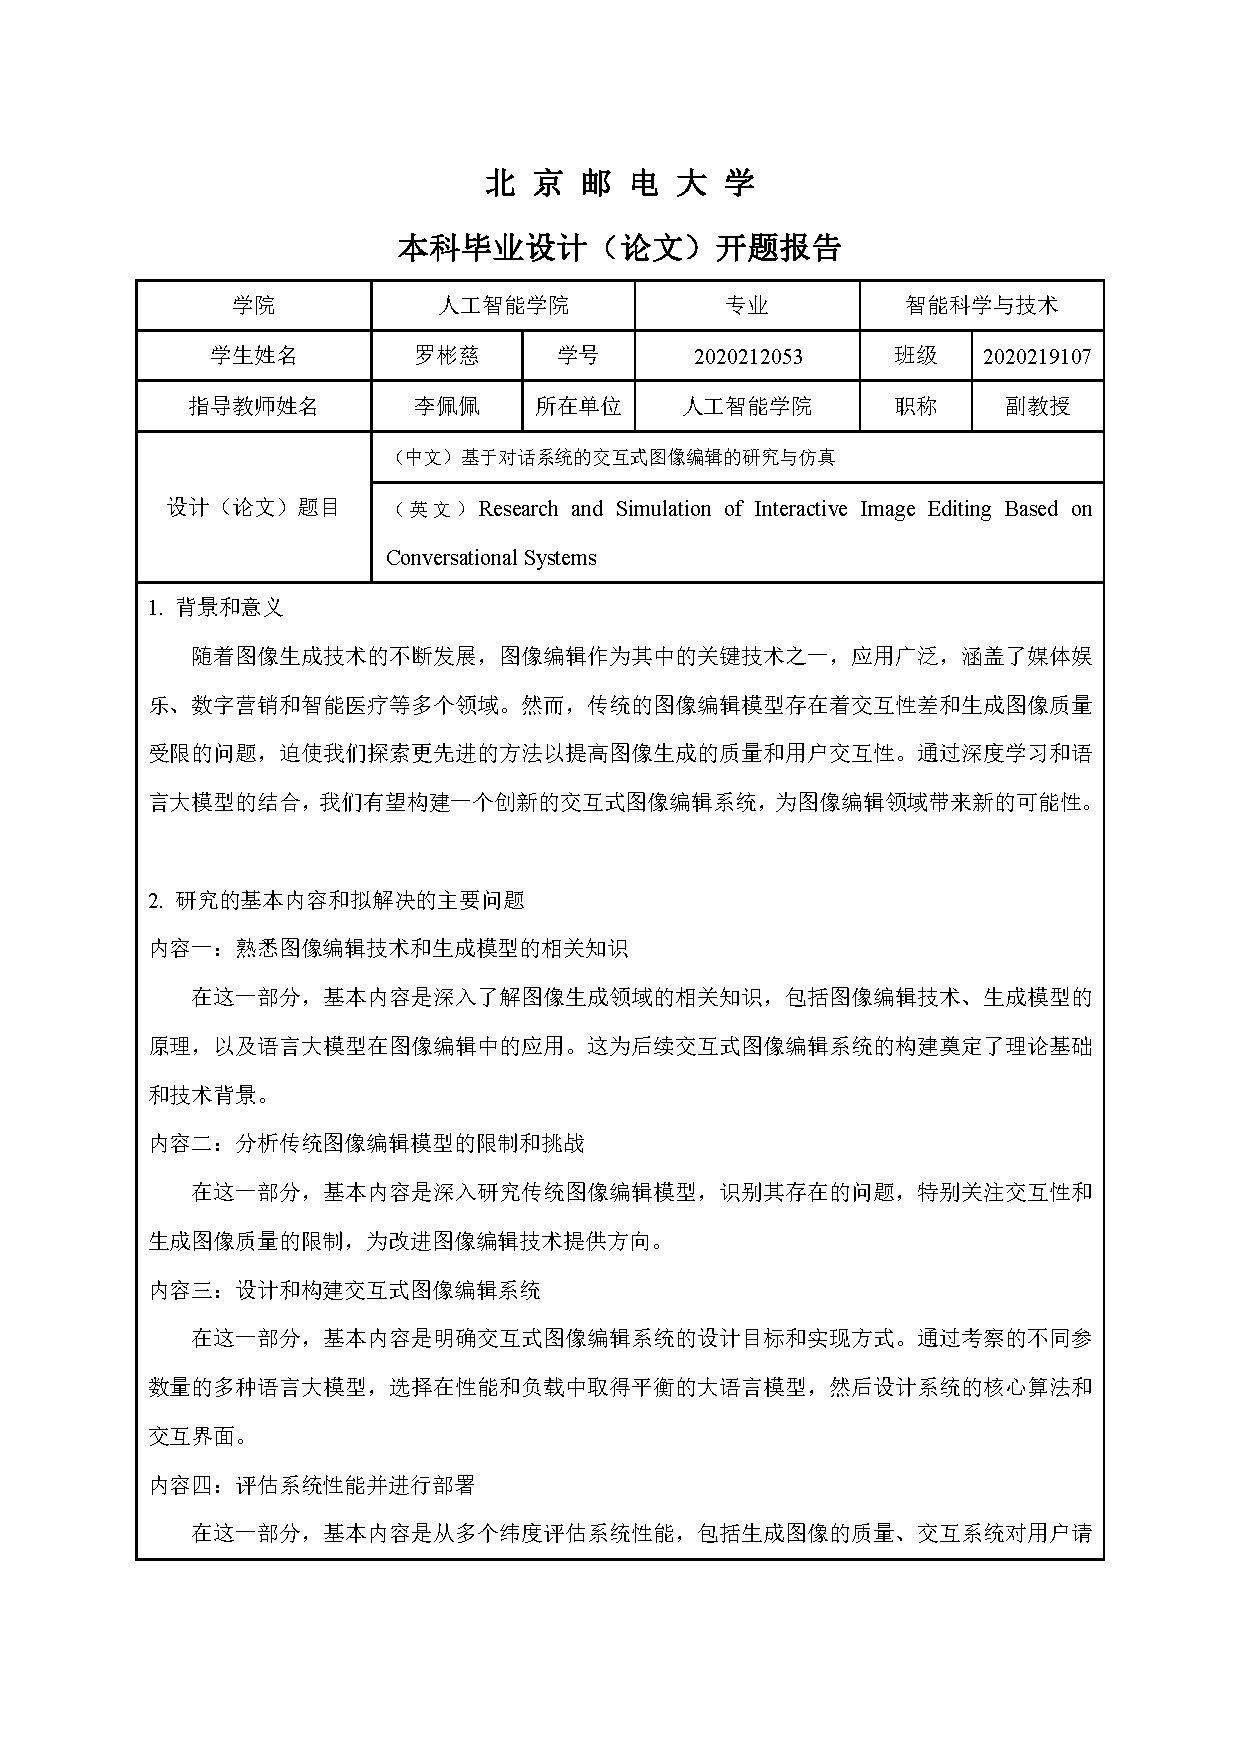
\includepdf[pages=-]{docs/openingReport.pdf}

% 中期检查表
\blankmatter
\phantomsection\addcontentsline{toc}{chapter}{中\quad{}期\quad{}检\quad{}查\quad{}表}
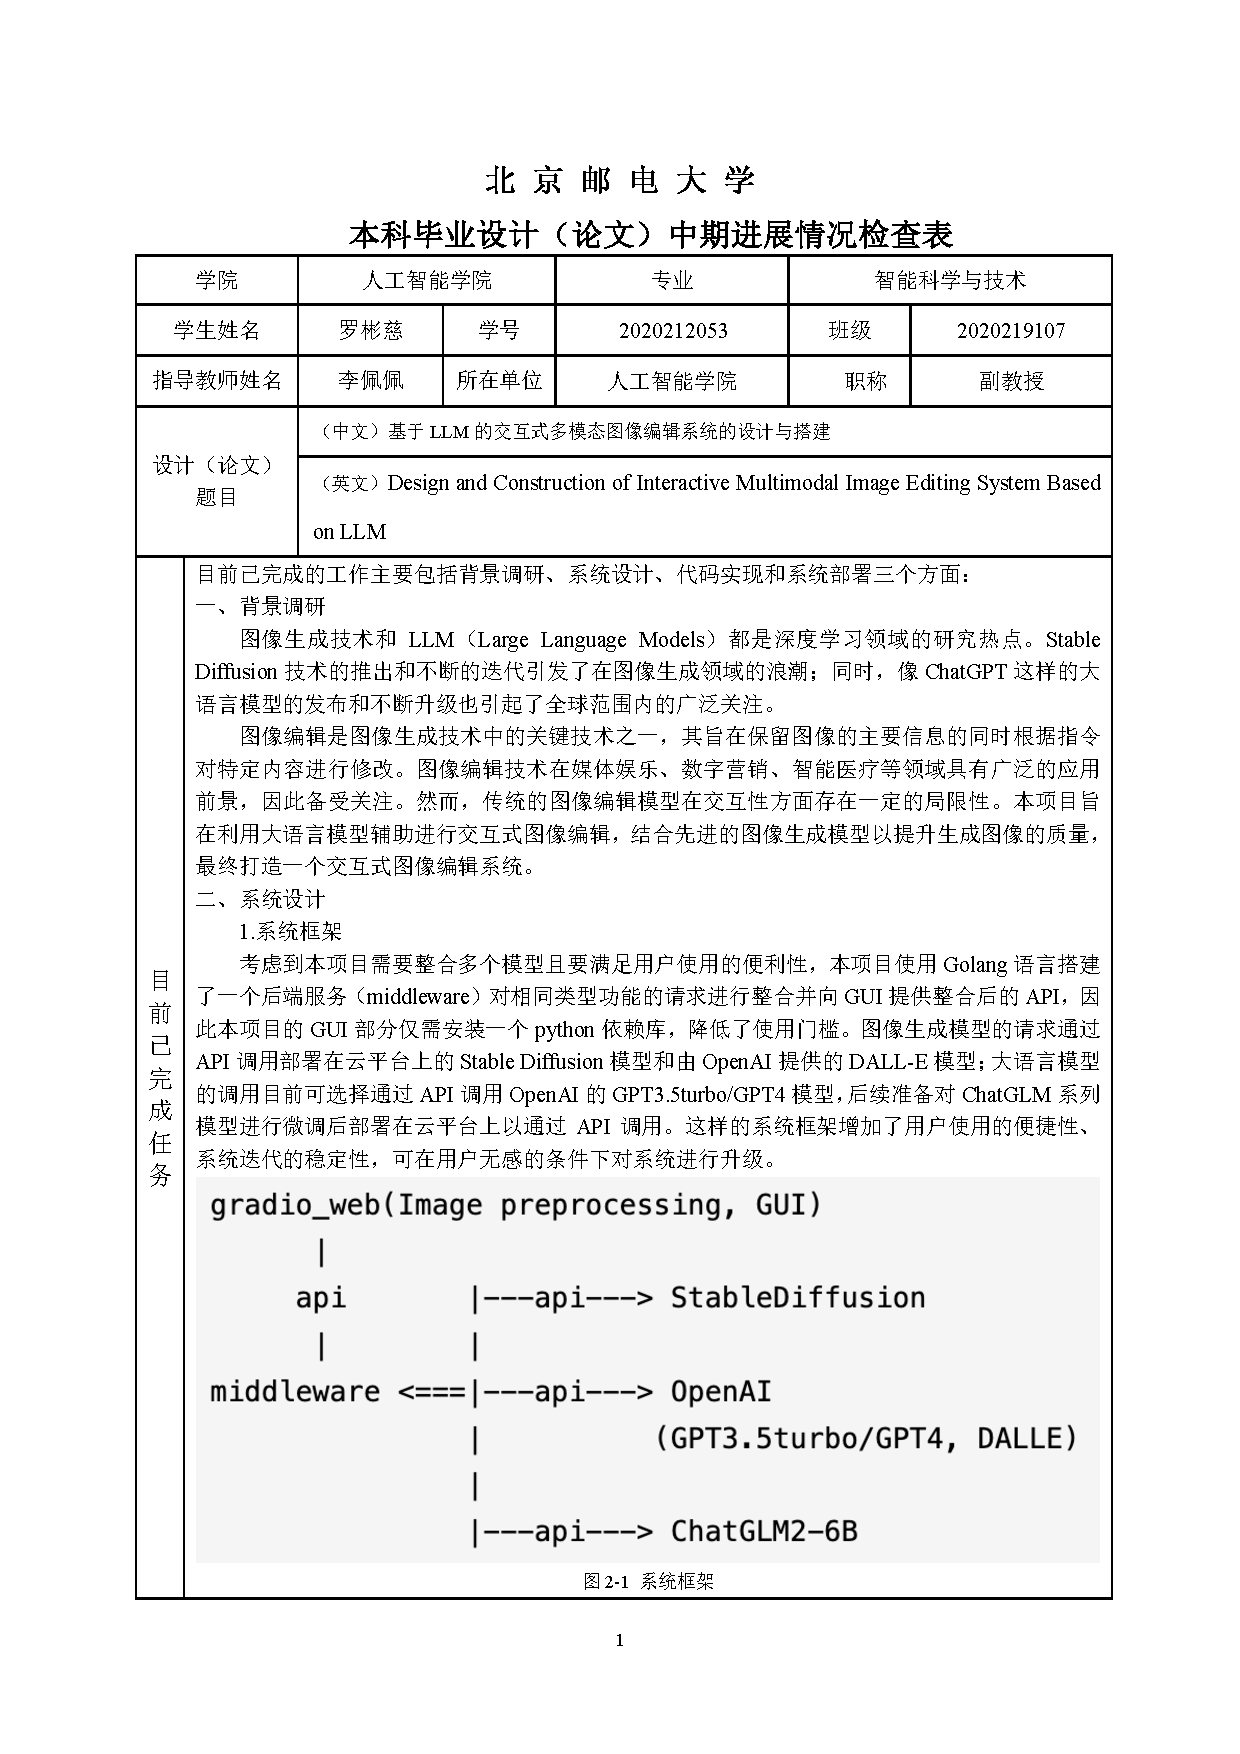
\includepdf[pages=-]{docs/interimReport.pdf}

% 教师指导毕业设计(论文)记录表
\blankmatter
\phantomsection\addcontentsline{toc}{chapter}{教师指导毕业设计(论文)记录表}

\includepdf[pages=-]{docs/guidance.pdf}

\end{nopagenumber}

\end{document}
